\chapter{Hacia un Framework Comparativo}
Android e iOS permiten cambiar ciertos permisos de una aplicación en tiempo de ejecución, es decir, luego de haberla instalado en el dispositivo. Para poner a prueba los sistemas de permisos de ambas plataformas, se ha desarrollado un framework que permite comparar formalmente diversos aspectos de seguridad.\\
El framework es una aplicación móvil y esta compuesto por varios tests. Cada test pone a prueba a un componente del dispositivo, permitiendo así conocer el alcance de los permisos correspondientes a dicho componente.\\
Todos los test fueron implementados en \emph{JavaScript} y corren en el dispositivo mediante \emph{Apache Cordova}\footnote{TODO: va la referencia hacia donde se explica que es Apache Cordova.}.\\
En las siguientes secciones se detallaran los distintos tests que componen el framework. Además, se mencionarán las conclusiones arribadas luego de correr los tests mencionados anteriormente.
\section{Vista principal}
Al iniciar la aplicación, lo primero que se observa son observan dos áreas principales: Acciones y Test.\\
La primera área contiene un botón para acceder a la configuración de los permisos del dispositivo. Allí, el \textit{tester} puede cambiar manualmente los permisos requeridos por la aplicación. Además, se encuentra un botón para limpiar la consola (que se encuentra en el otro área).\\
Mientras que la segunda área se subdivide en dos: en la parte de los tests y la parte de la consola. Una parte corresponde a los botones de los tests que, al presionarse, ejecutan el respectivo test, mostrando en la consola el resultado. Dicho resultado se mostrara con tipografía color verde si fue exitoso; en cambio, se mostrara con tipografía color roja de ser fallido.\\
\begin{figure}[hbtp]
    \centering
	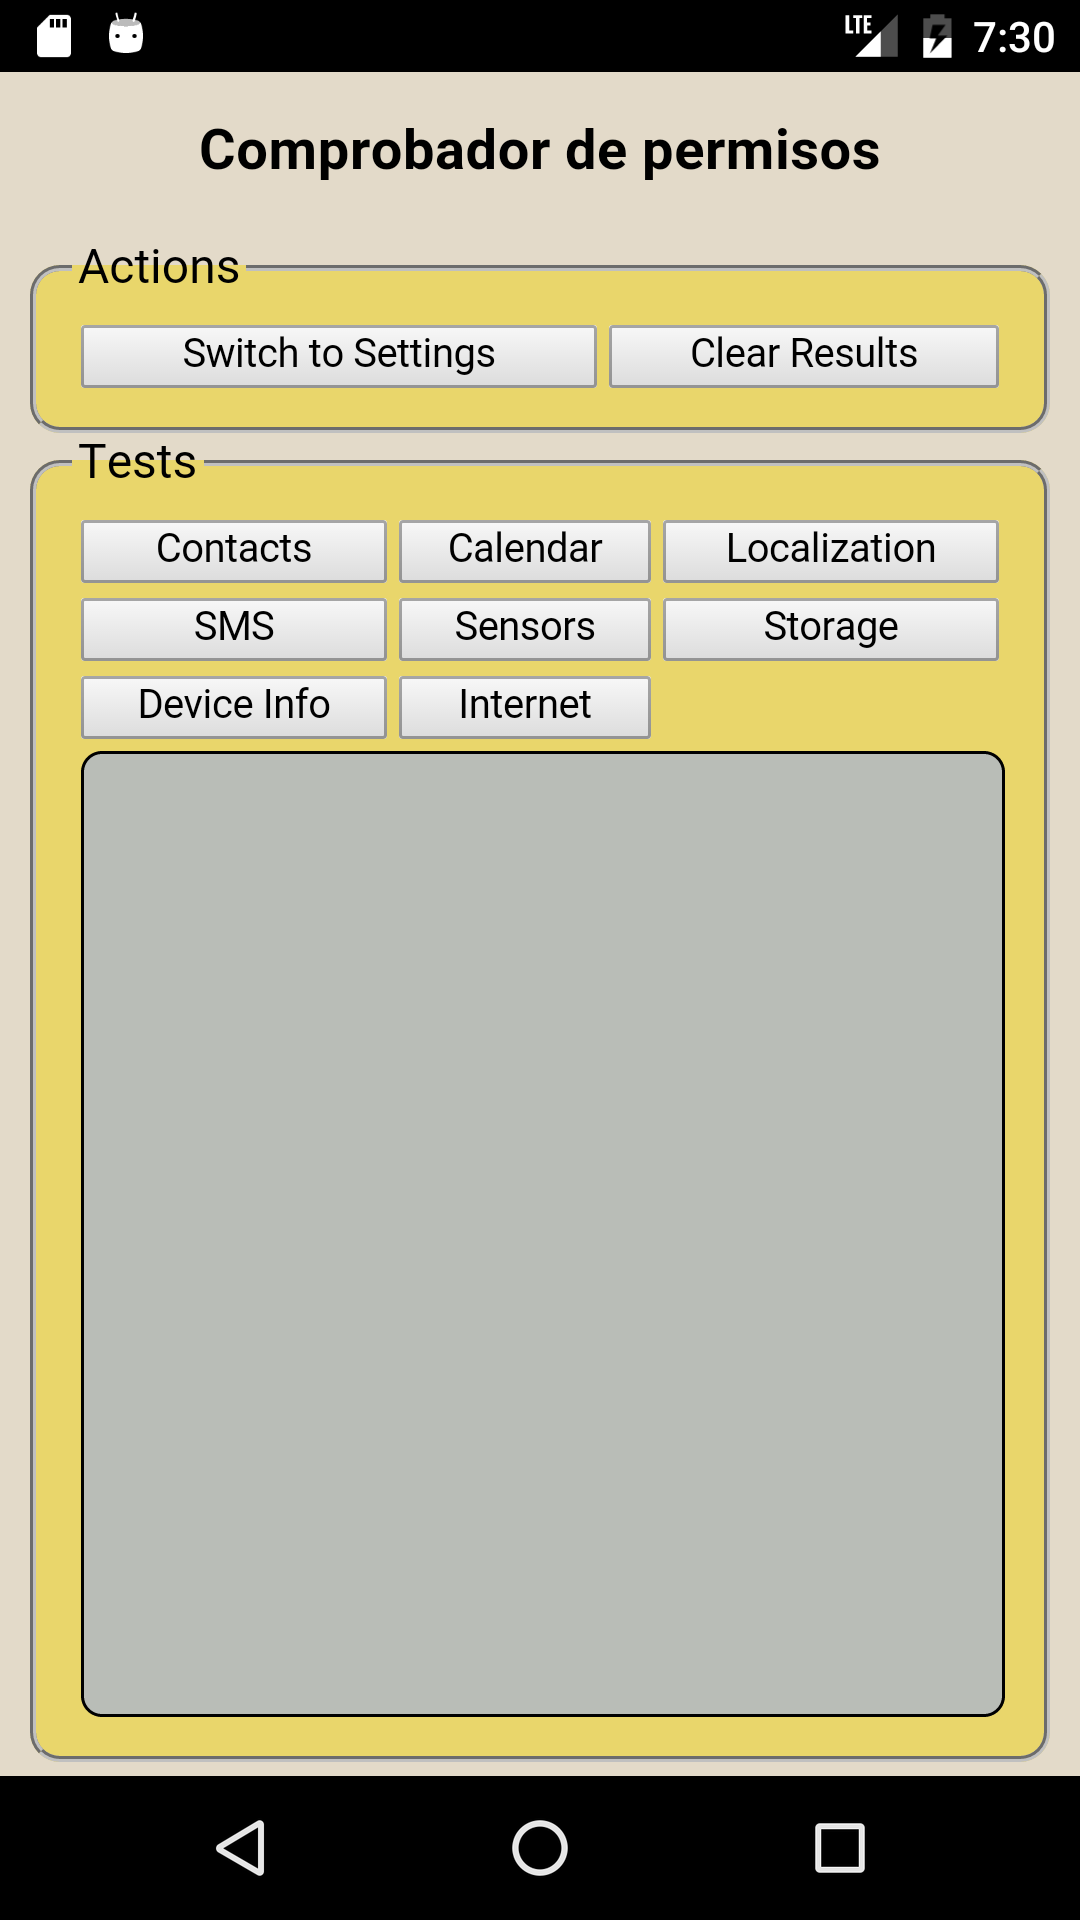
\includegraphics[width=0.4\linewidth]{chapter5/app_main_view}
	\caption{Áreas de la aplicación \textit{Runtime Permissions Test}.}
	\label{fig:chapter05:main_view}
\end{figure}
En la Figura \ref{fig:chapter05:main_view} se observan las áreas del framework.\\

A continuación se mencionan los componentes que se pueden testear con el framework:
\begin{itemize}
	\item Contactos
	\item Calendario
	\item Localización
	\item SMS
	\item Sensores
	\item Almacenamiento
	%\item AppAvaiable (funciona en ambos) Es medio tonto. Probar si detecta mi app...
	\item Información del dispositivo.
	\item Acceso a Internet
	%\item Bateria (falta)
	%\item Health (falta - solo en iOS)
\end{itemize}
%\textbf{\emph{Plugin:}} \href{https://www.npmjs.com/package/cordova.plugins.diagnostic}{cordova.plugins.diagnostic v3.1.7}\\
\subsection{Funciones no compatibles}
El emulador ofical de Android es compatible con la mayoría de las funciones de un dispositivo, pero no incluye la posibilidad de virtualizar los siguientes componentes \cite{daemu}:
\begin{itemize}
    \item WiFi;
    \item Bluetooth;
    \item NFC\footnote{Del ingles \emph{Near Field Communication}. Es una tecnología de comunicación inalámbrica, de corto alcance y alta frecuencia que permite el intercambio de datos entre dispositivos.};
    \item Manipulación de la tarjeta SD;
    \item Conexión USB;
    \item Micrófono;
    \item Cámara
\end{itemize}
Al no poder manipular la tarjeta SD, no es posible testear ninguna las funcionalidades multimedia: no se pueden grabar audio, ni video ni sacar fotos.\\
Por lo tanto, no se agregaron al framework tests para los componentes listados anteriormente.
\section{C\'atalogo de test}
En esta sección se listaran todos los test que conforman al framework. Para cada test se detallara su algoritmo, los plugins de Apache Cordova que se utilizaron para confeccionarlo y una serie de capturas.
\subsection{Calendario}
\textbf{\emph{Plugin:}} \href{https://www.npmjs.com/package/cordova-plugin-calendar}{cordova-plugin-calendar v4.5.5}
\begin{algorithm}
	\begin{algorithmic}[1]
		\STATE se crea la fecha $startDate$
		\STATE se crea la fecha $endDate$
		\STATE se crea un evento que empieza en la fecha $startDate$ y termina en la fecha $endDate$.
		\STATE se listan los eventos entre las fechas $startDate$ y $endDate$.
	\end{algorithmic}
	\caption{Test de los permisos del calendario}\label{alg:chap5:test_calendario}
\end{algorithm}

\begin{figure}[hbtp]
    \centering
    \begin{subfigure}{0.3\linewidth}
        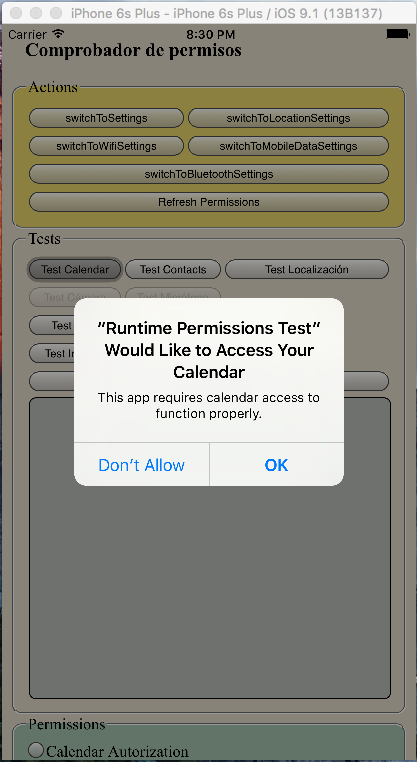
\includegraphics[width=\linewidth]{chapter5/calendar_request_ios}
    \end{subfigure}
    \begin{subfigure}{0.3\linewidth}
        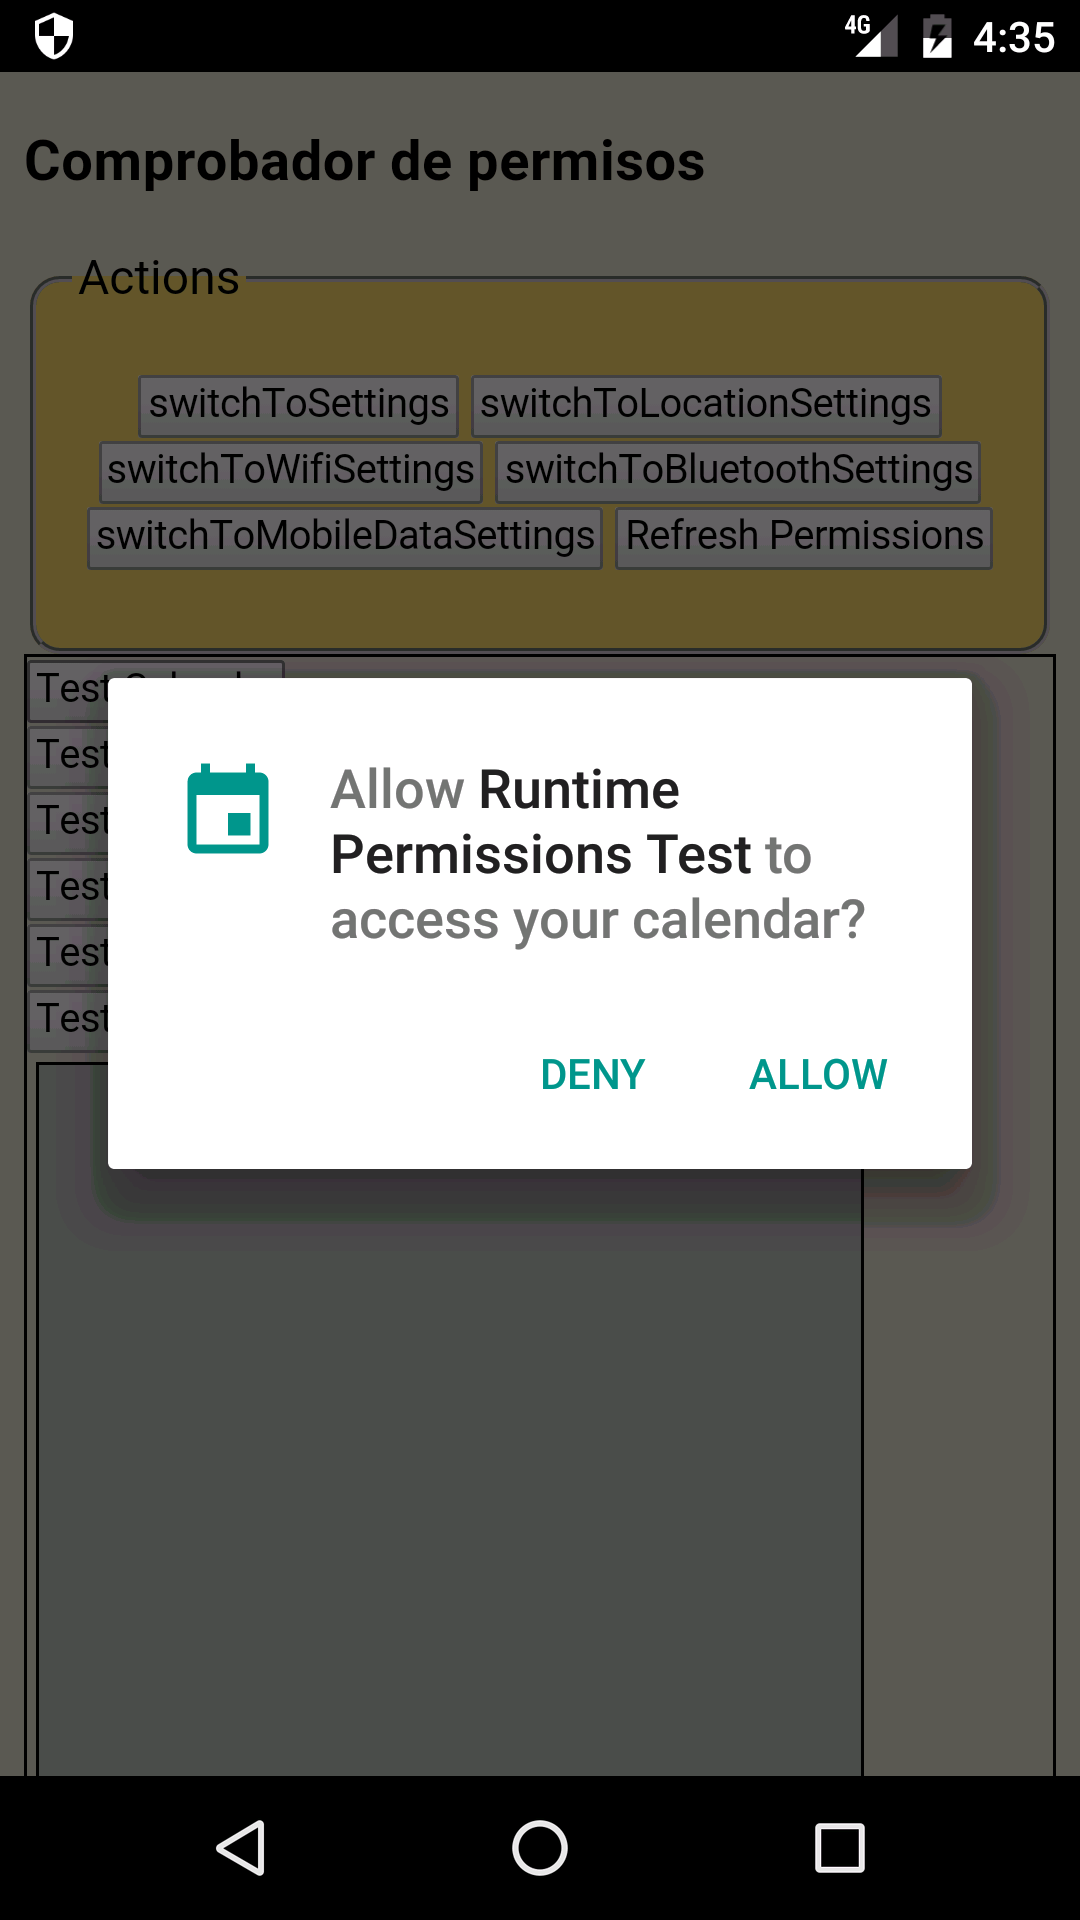
\includegraphics[width=\linewidth]{chapter5/allow_calendar}
    \end{subfigure}
    \caption{Captura del momento en que se requiere un permiso para las distintas plataformas.}
	\label{fig:ch05:app-permissions-allow}
\end{figure}
\begin{figure}[hbtp]
    \centering
    \begin{subfigure}{0.3\linewidth}
        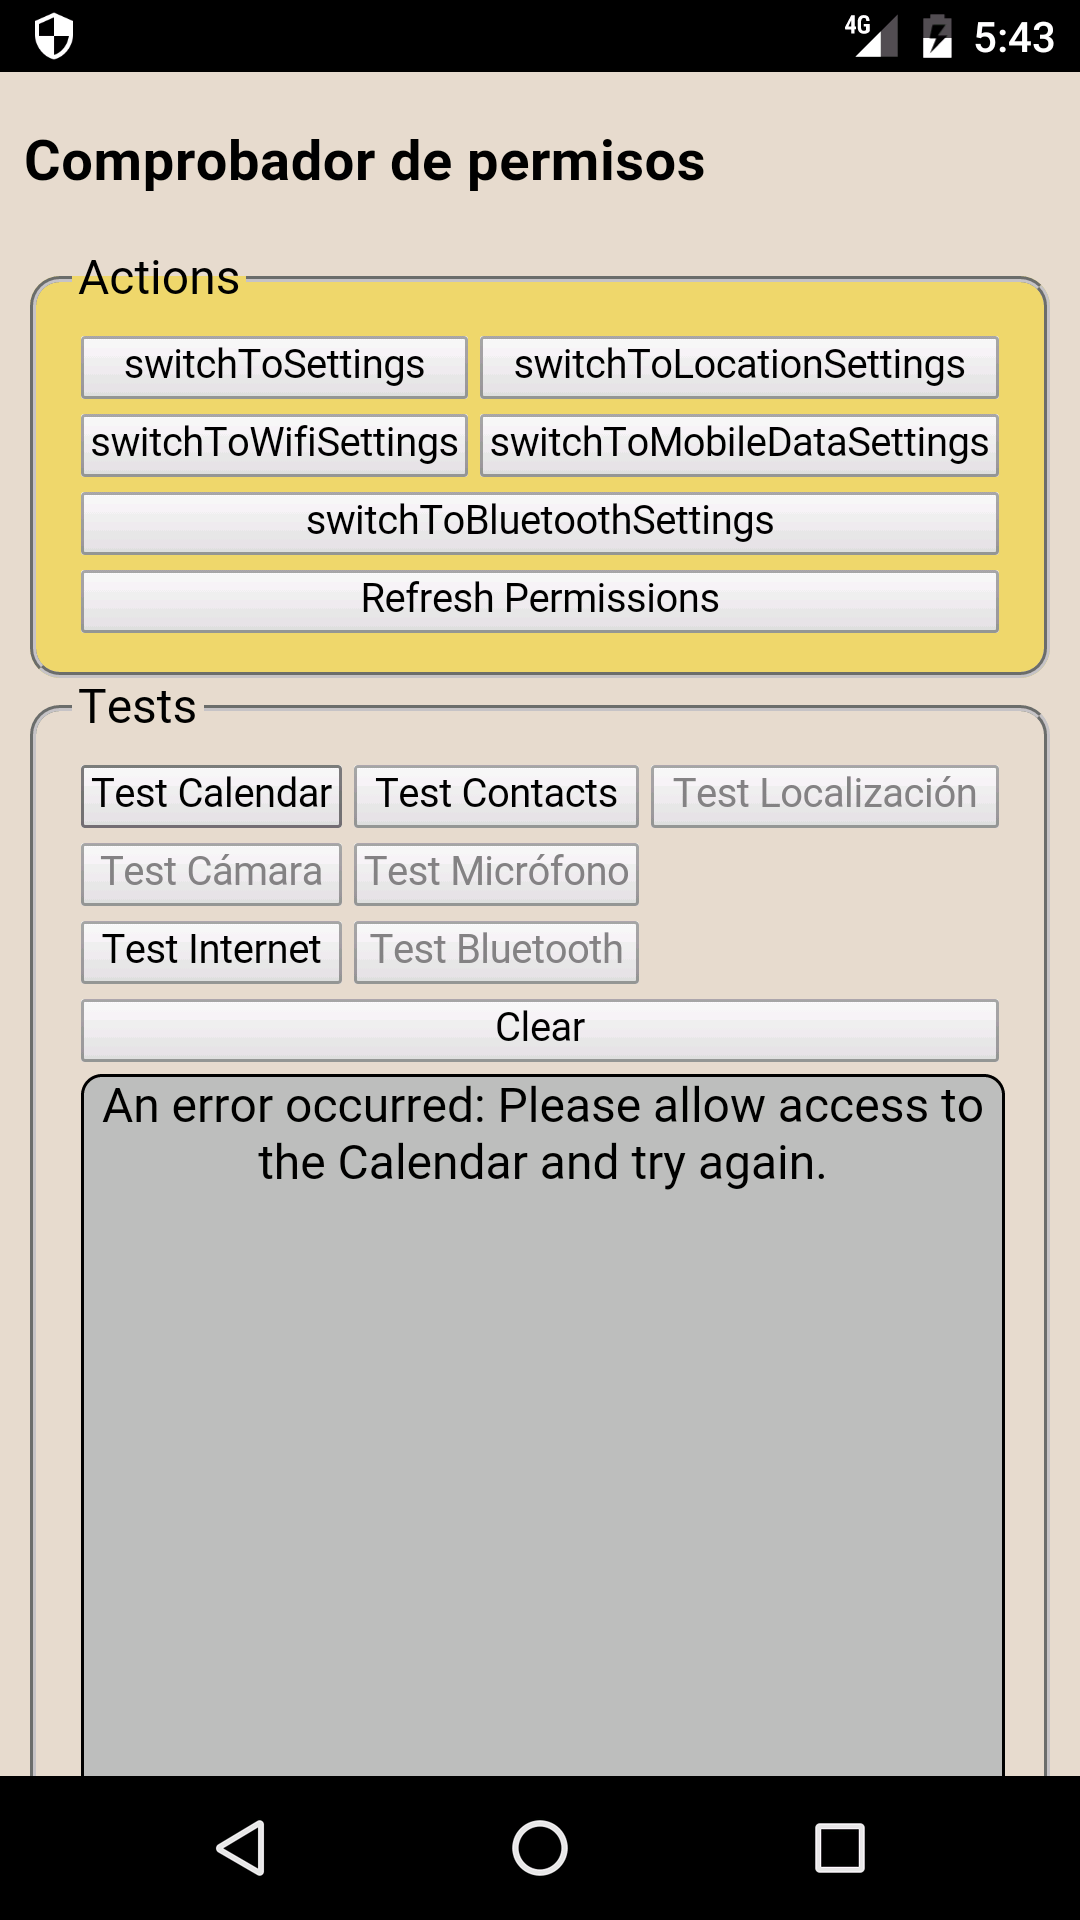
\includegraphics[width=\linewidth]{chapter5/without_calendar}
        \label{fig:chapter05:without_calendar}
    \end{subfigure}
    \begin{subfigure}{0.3\linewidth}
        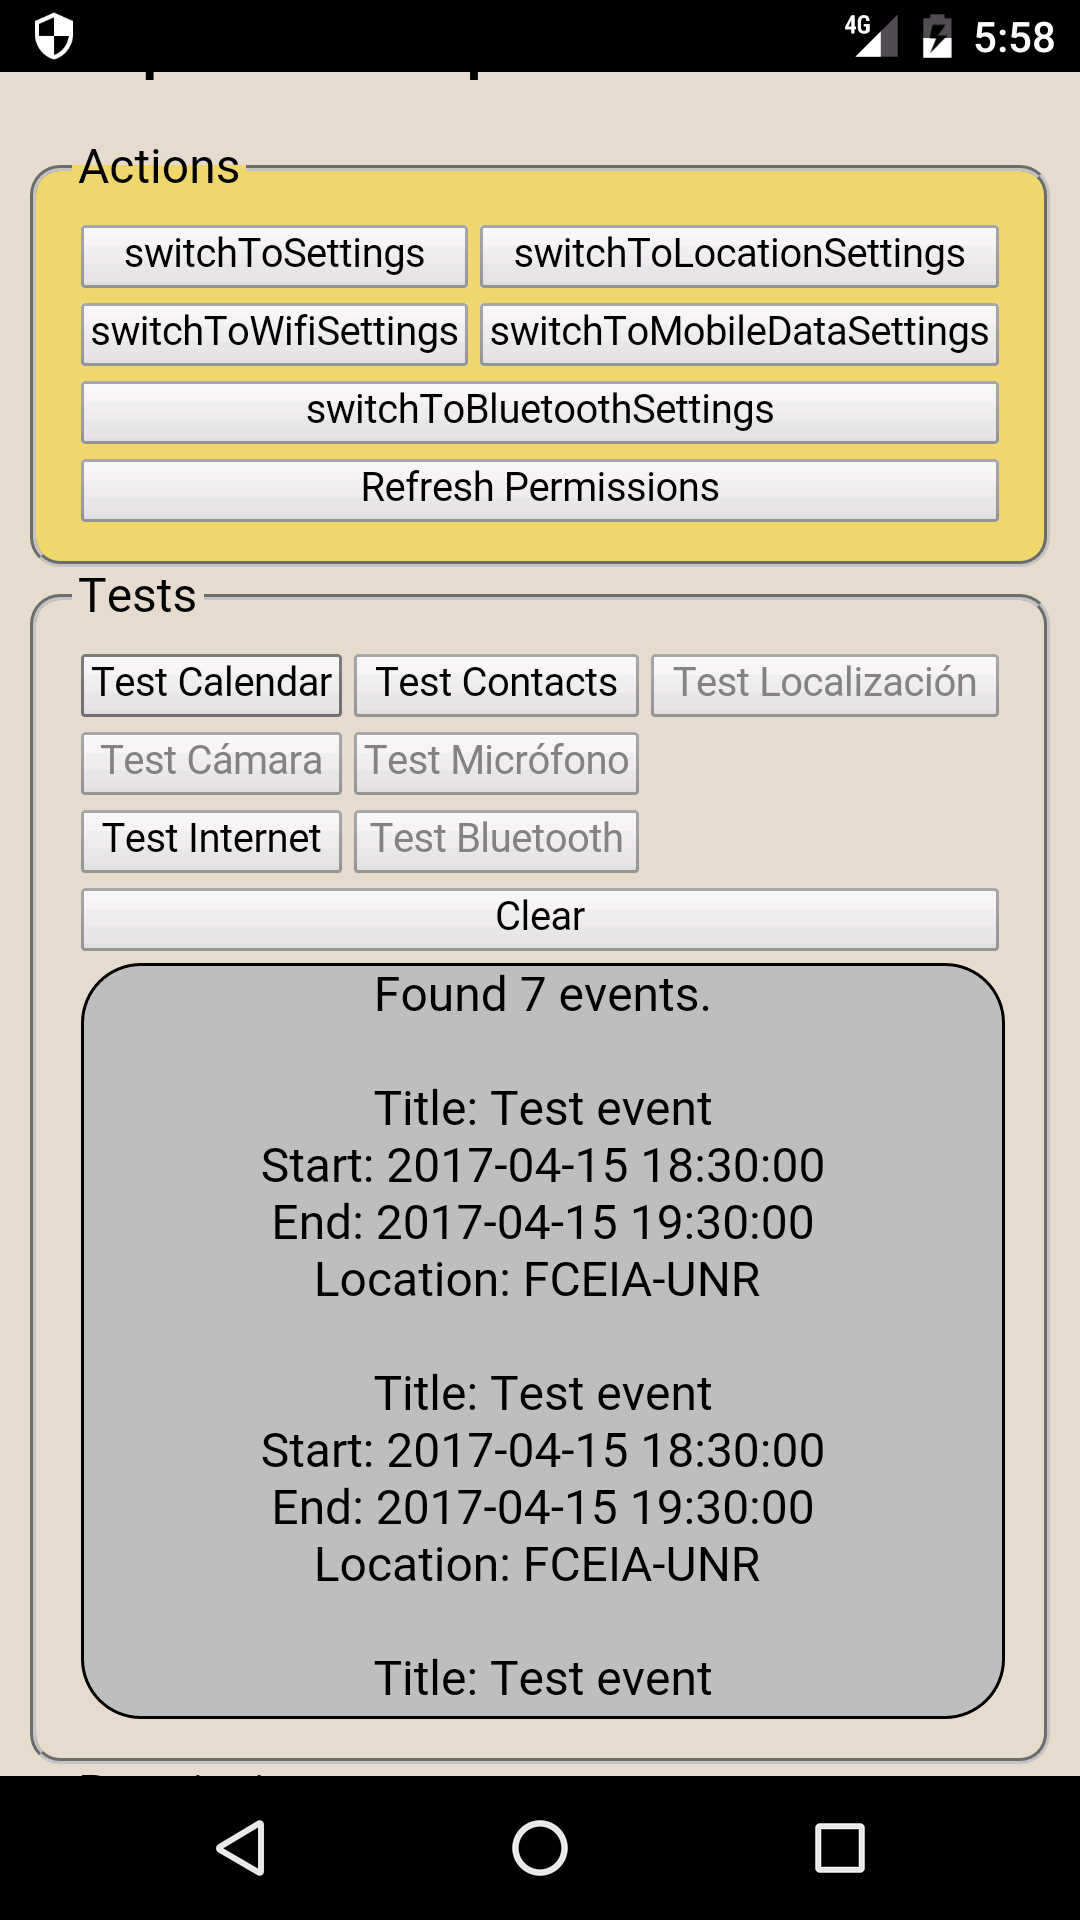
\includegraphics[width=\linewidth]{chapter5/with_calendar}
        \label{fig:chapter05:with_calendar}
    \end{subfigure}
    \caption{Caso exitoso y caso fallido.}
	\label{fig:ch05:calendar-cases}
\end{figure}
\newpage
\subsection{Contactos}
\textbf{\emph{Plugin:}} \href{https://www.npmjs.com/package/cordova-plugin-contacts}{cordova-plugin-contacts v2.2.1}
\begin{algorithm}
	\begin{algorithmic}[1]
		\STATE se listan todos los contactos.
		\STATE se crea un nuevo contacto.
		\STATE se listan todos los contactos.
	\end{algorithmic}
	\caption{Test de los permisos de los contactos}\label{alg:chap5:test_contactos}
\end{algorithm}
\begin{figure}[!ht]
	\begin{subfigure}{.24\textwidth}
	    \centering
		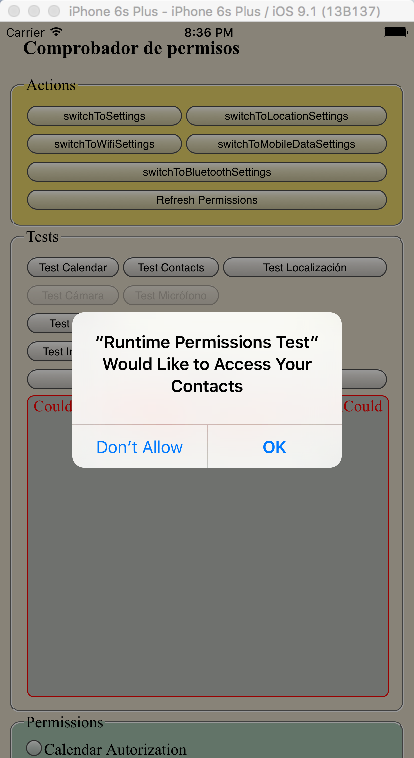
\includegraphics[width=3.75cm]{chapter5/contacts_request_ios}
		\label{fig:chapter05:allow_contact_ios}
	\end{subfigure}
	\begin{subfigure}{.24\textwidth}
	    \centering
		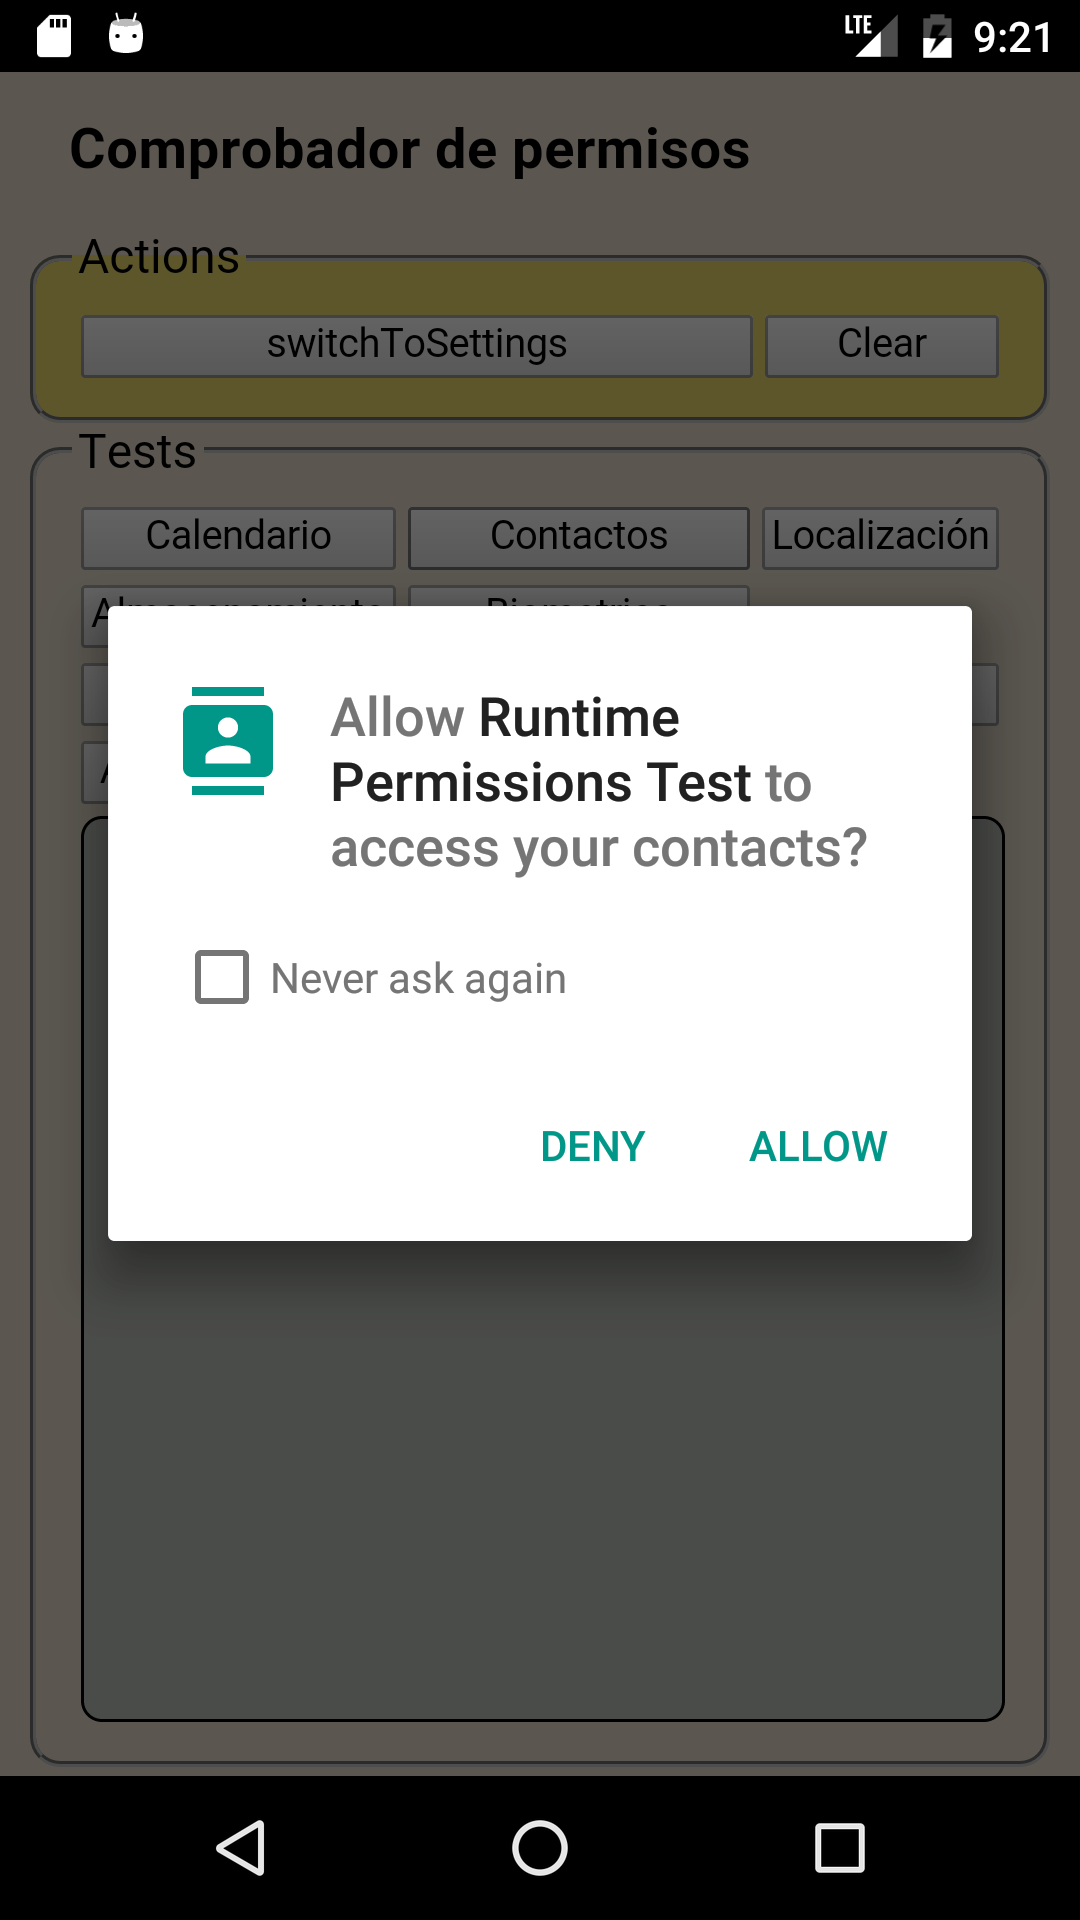
\includegraphics[width=3.75cm]{chapter5/allow_contact}
		\label{fig:chapter05:allow_contact_android}
	\end{subfigure}		
	\begin{subfigure}{.25\textwidth}
	    \centering
		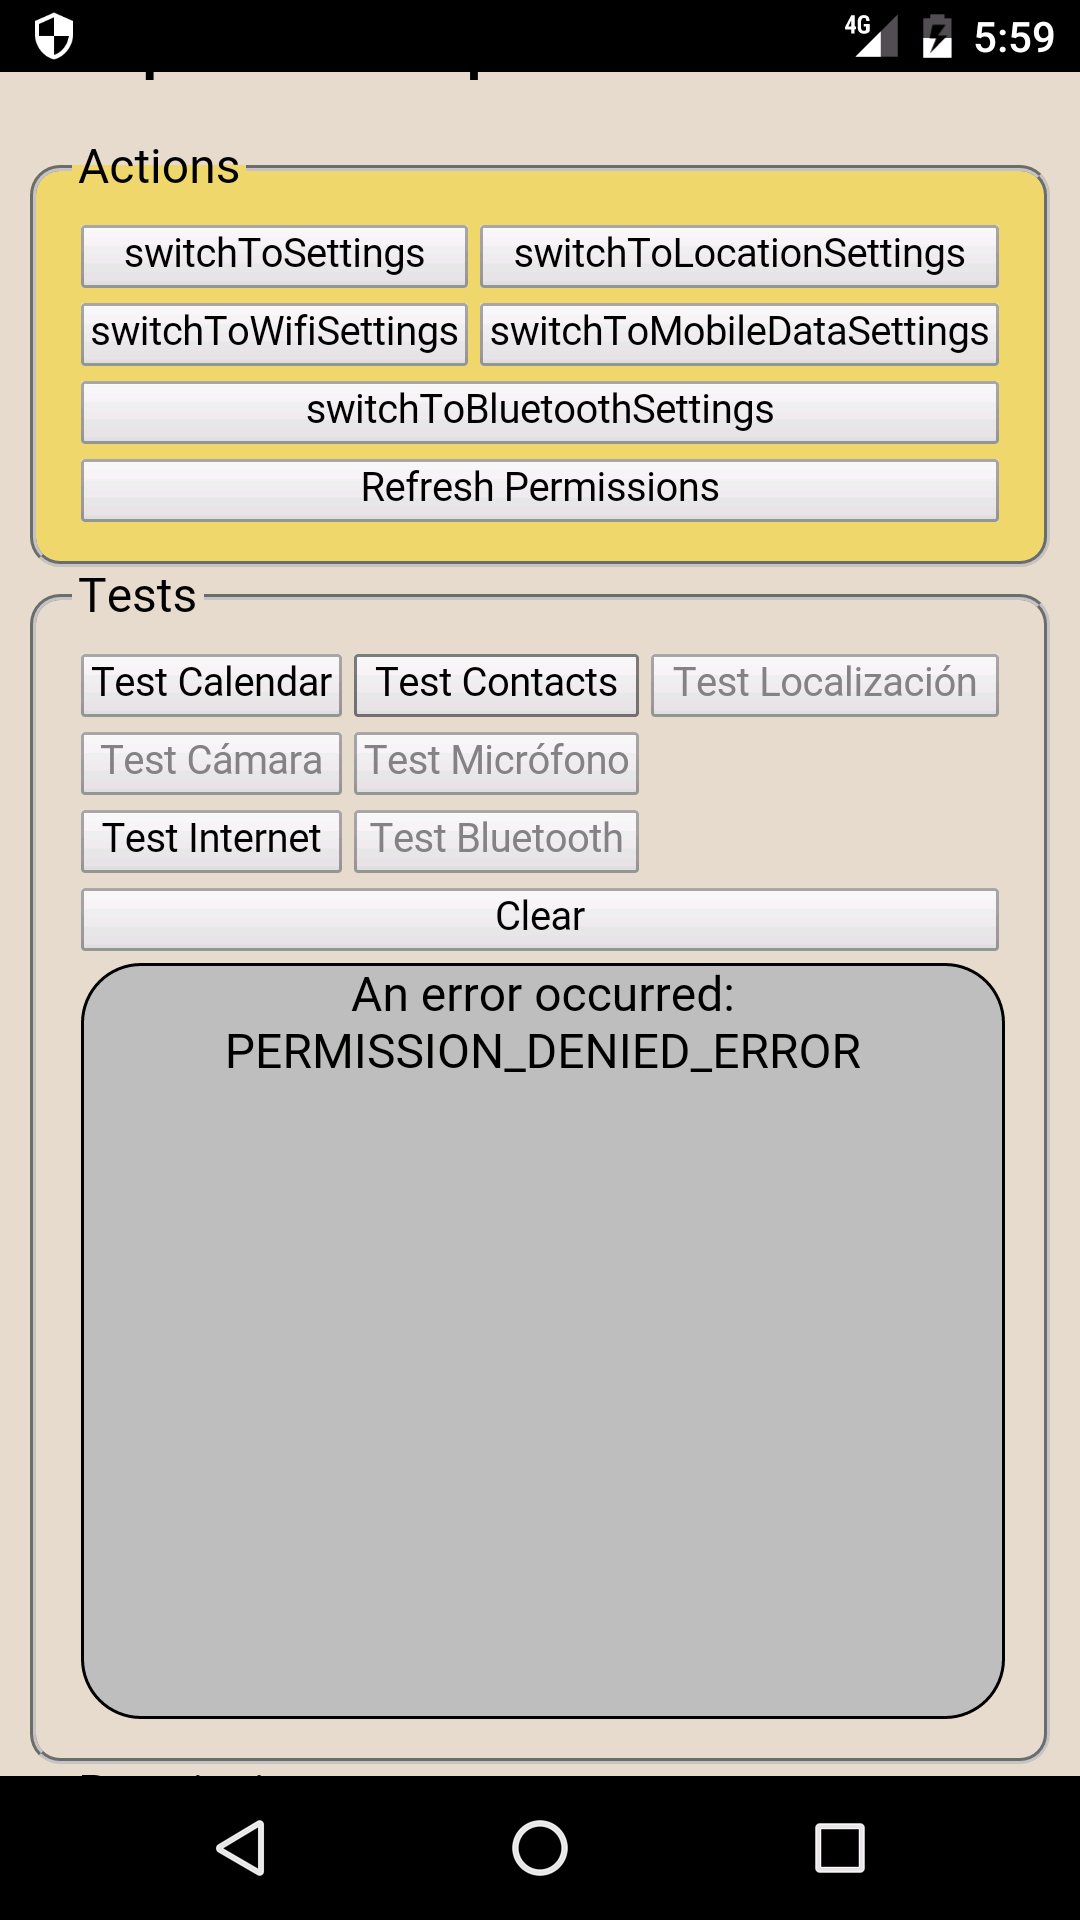
\includegraphics[width=3.75cm]{chapter5/without_contact}
		\label{fig:chapter05:without_contact}
	\end{subfigure}
	\begin{subfigure}{.25\textwidth}
	    \centering
		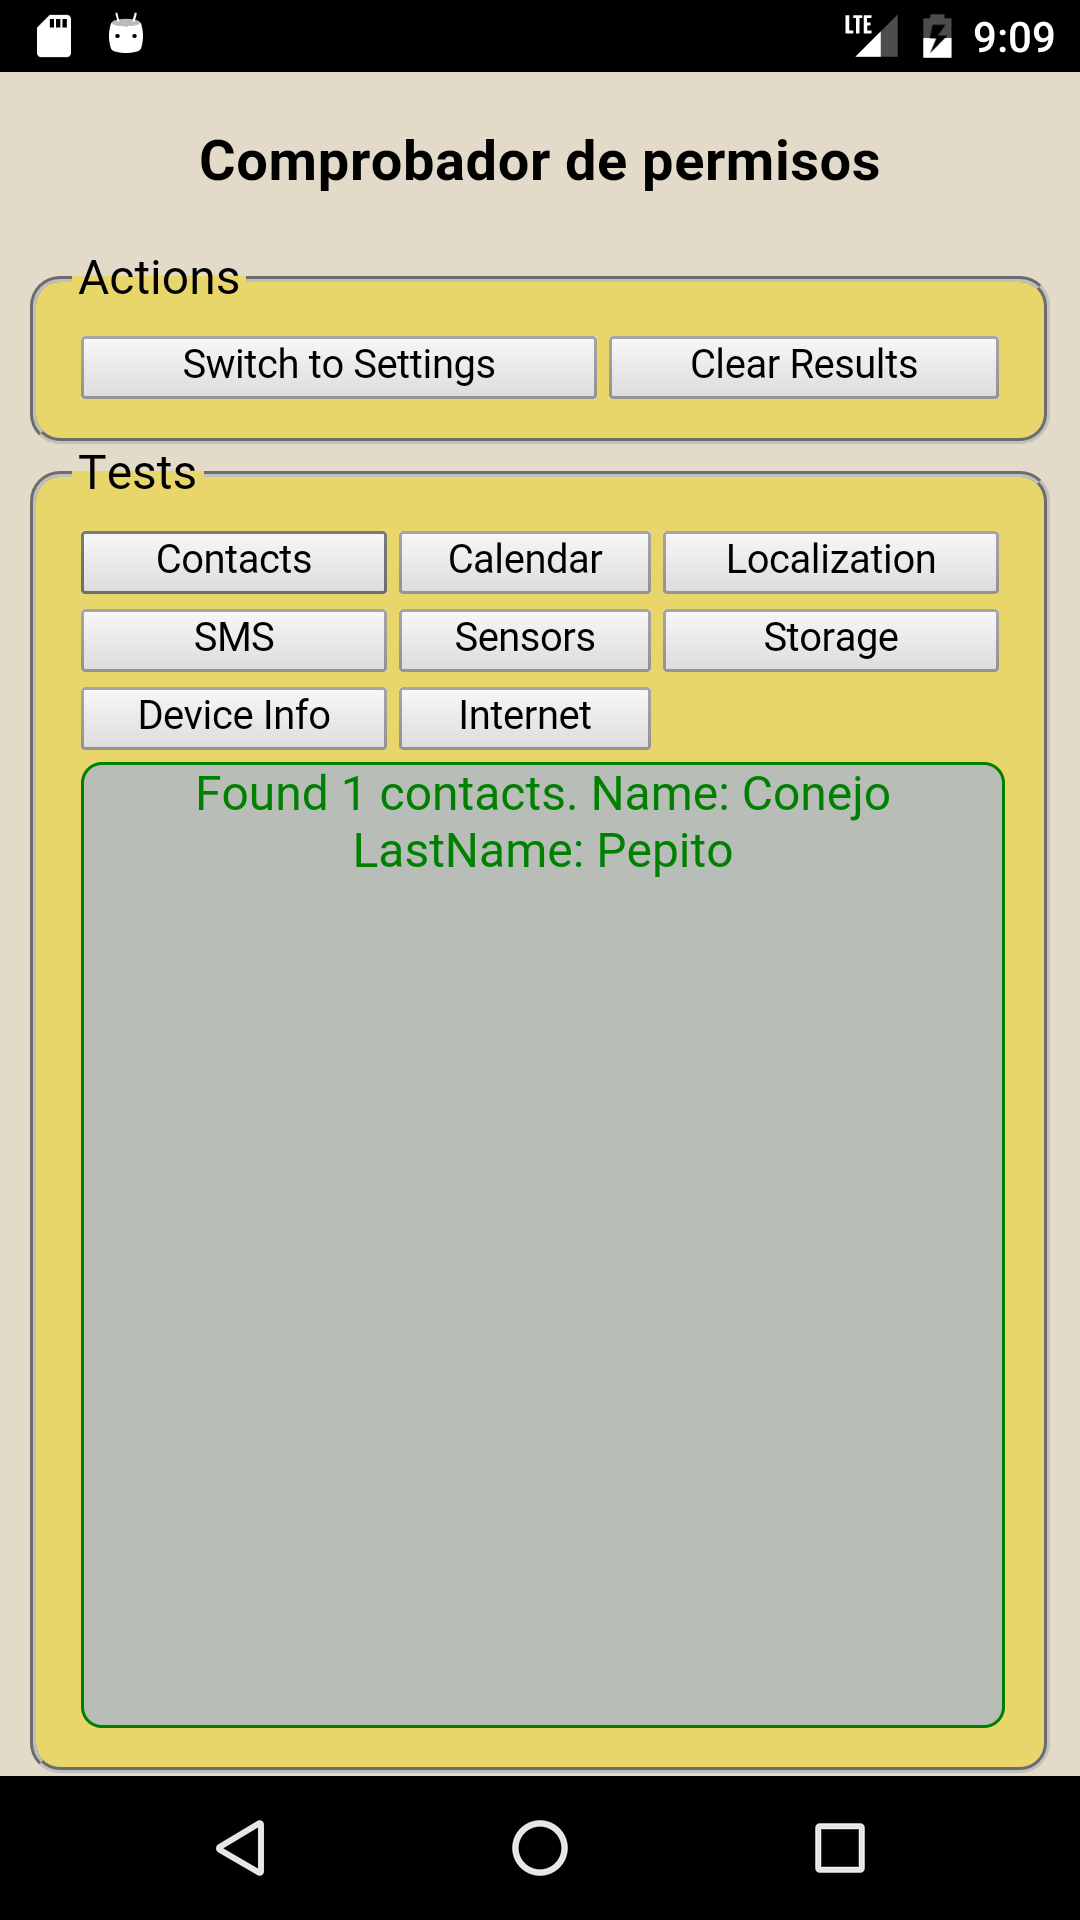
\includegraphics[width=3.75cm]{chapter5/with_contact}
		\label{fig:chapter05:with_contact}
	\end{subfigure}
	\caption{Testeando la administraci\'on de los contactos}
	\label{fig:chapter05:contact_test}
\end{figure}
\newpage
\subsection*{Geolocalización}
\textbf{\emph{Plugin:}} \href{https://github.com/apache/cordova-plugin-geolocation}{cordova-plugin-geolocation v2.4.3}\\
\begin{figure}[!ht]
    \centering
	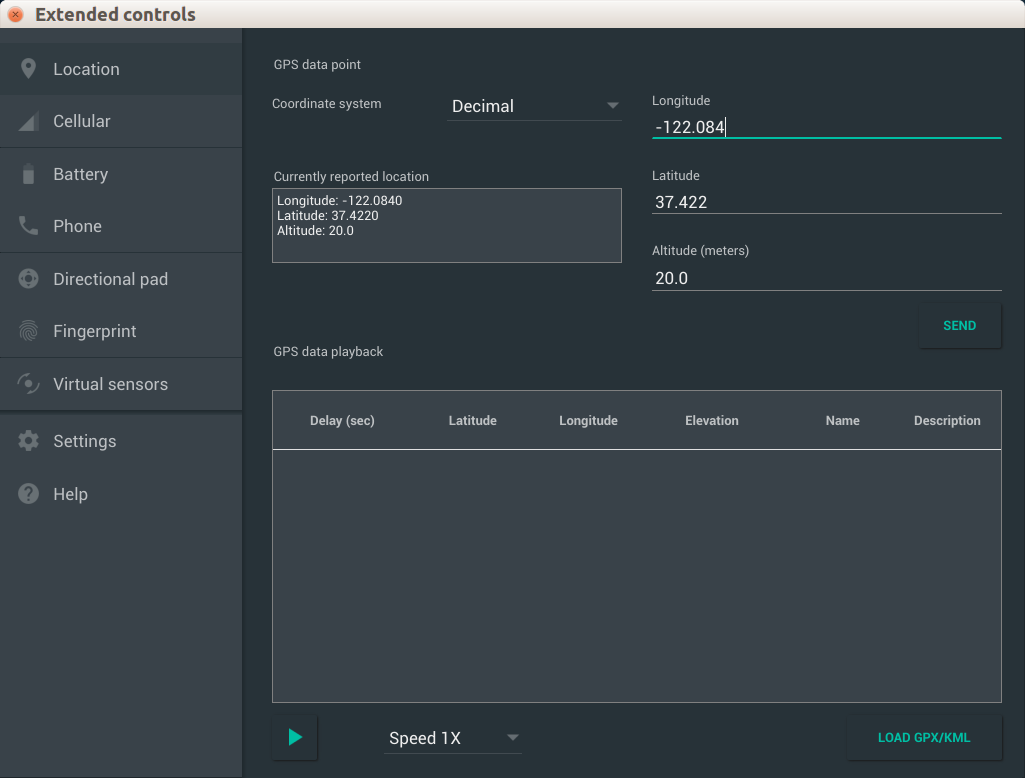
\includegraphics[width=8cm]{chapter5/android_extended_controls}
	\caption{Se pueden observar las coordenadas que se emulan.}
	\label{fig:chapter05:android_extended_controls}
\end{figure}
Desde el emulador, se simula unas coordenadas (Figura \ref{fig:chapter05:android_extended_controls}). Mediante el plugin utilizado, se obtienen los datos, siempre y cuando se tengan los permisos correspondientes. En la Figura \ref{fig:chapter05:geolocation_test} se observa lo mencionado anteriormente. El test simplemente consiste en pedir las coordenadas actuales.
\begin{figure}[!ht]
	\begin{subfigure}{.24\textwidth}
	    \centering
		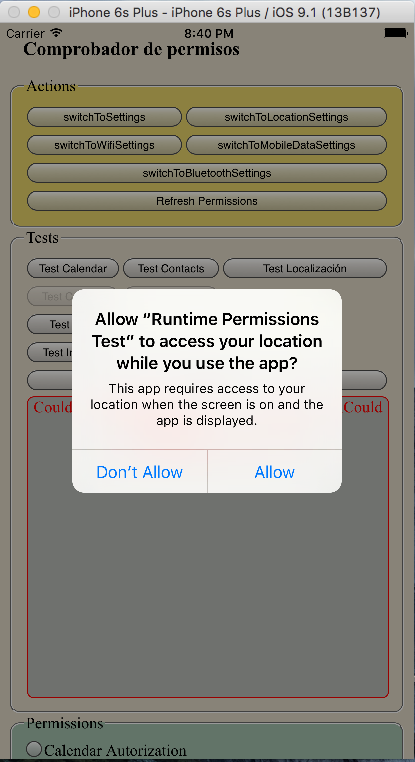
\includegraphics[width=3.75cm]{chapter5/location_request_ios}
		\label{fig:chapter05:allow_location_ios}
	\end{subfigure}
	\begin{subfigure}{.24\textwidth}
	    \centering
		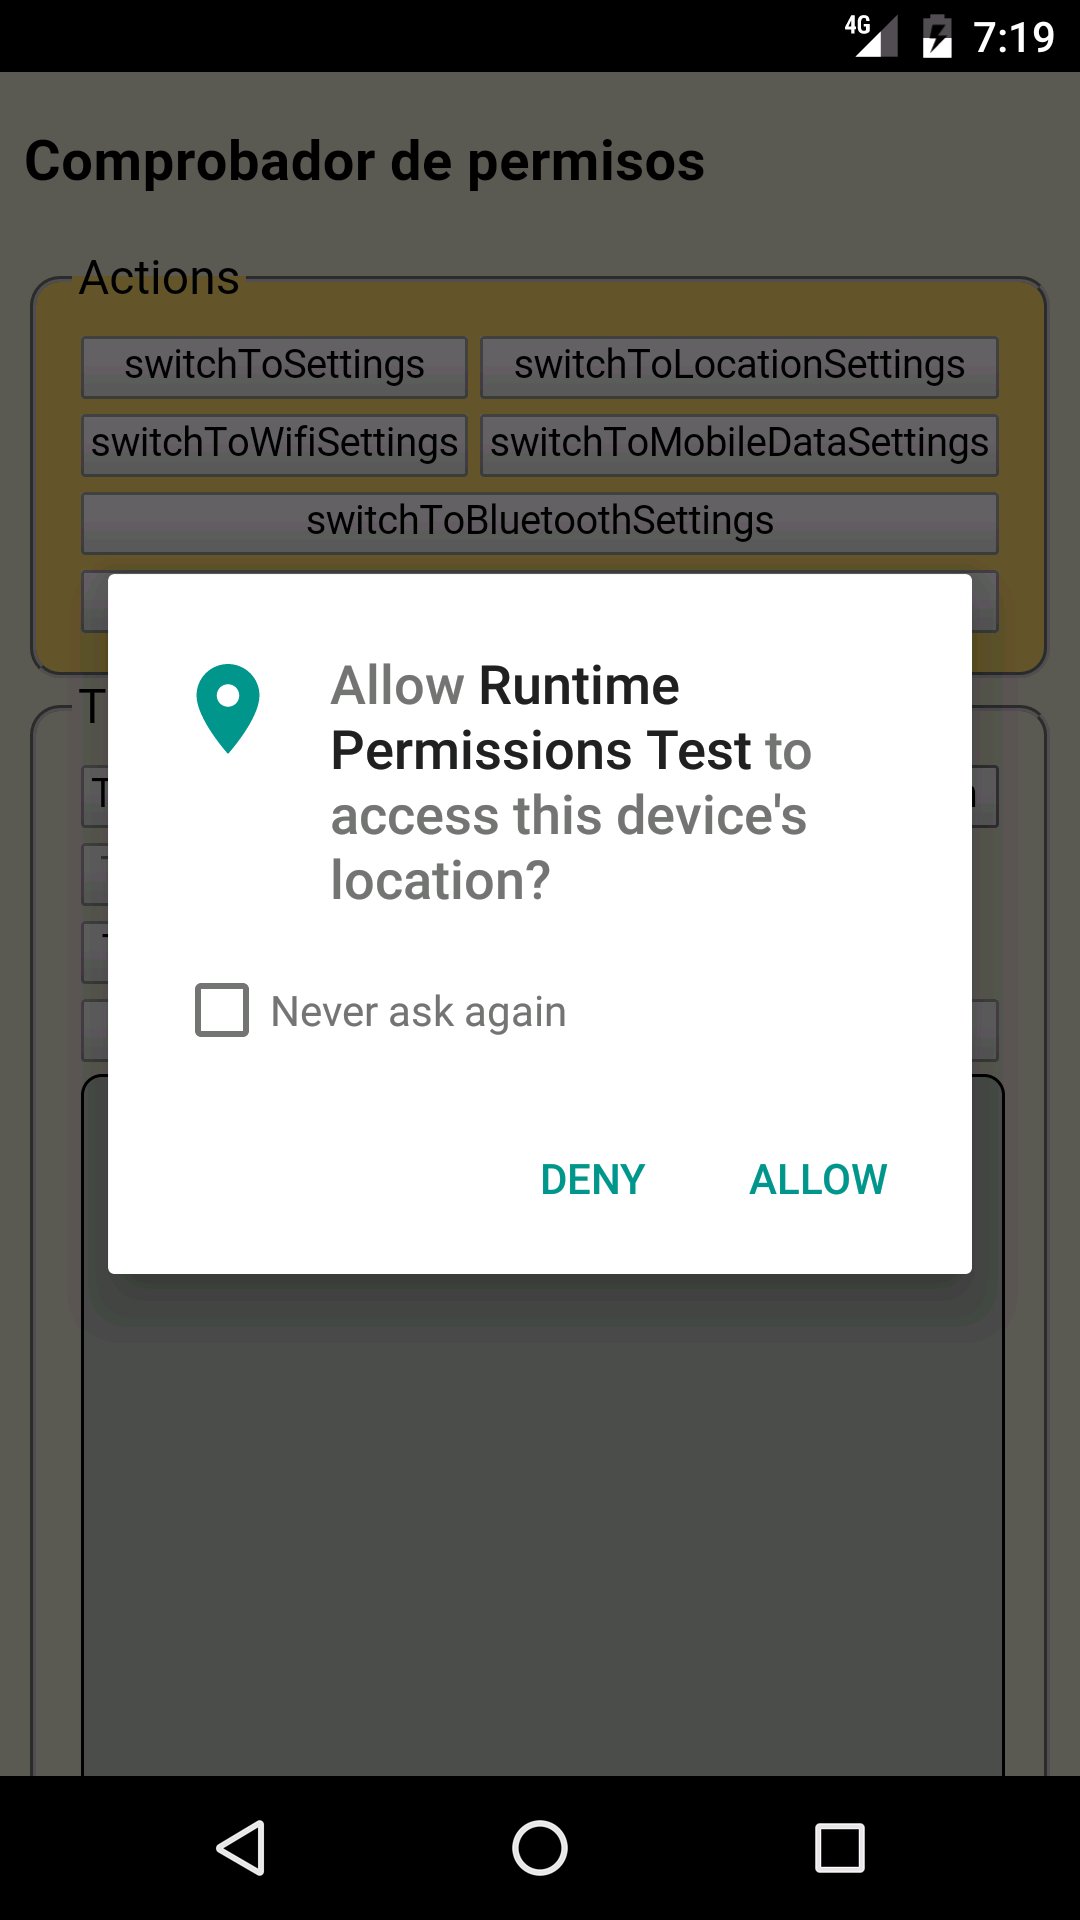
\includegraphics[width=3.75cm]{chapter5/allow_location}
		\label{fig:chapter05:allow_location_android}
	\end{subfigure}
	\begin{subfigure}{.24\textwidth}
	    \centering
		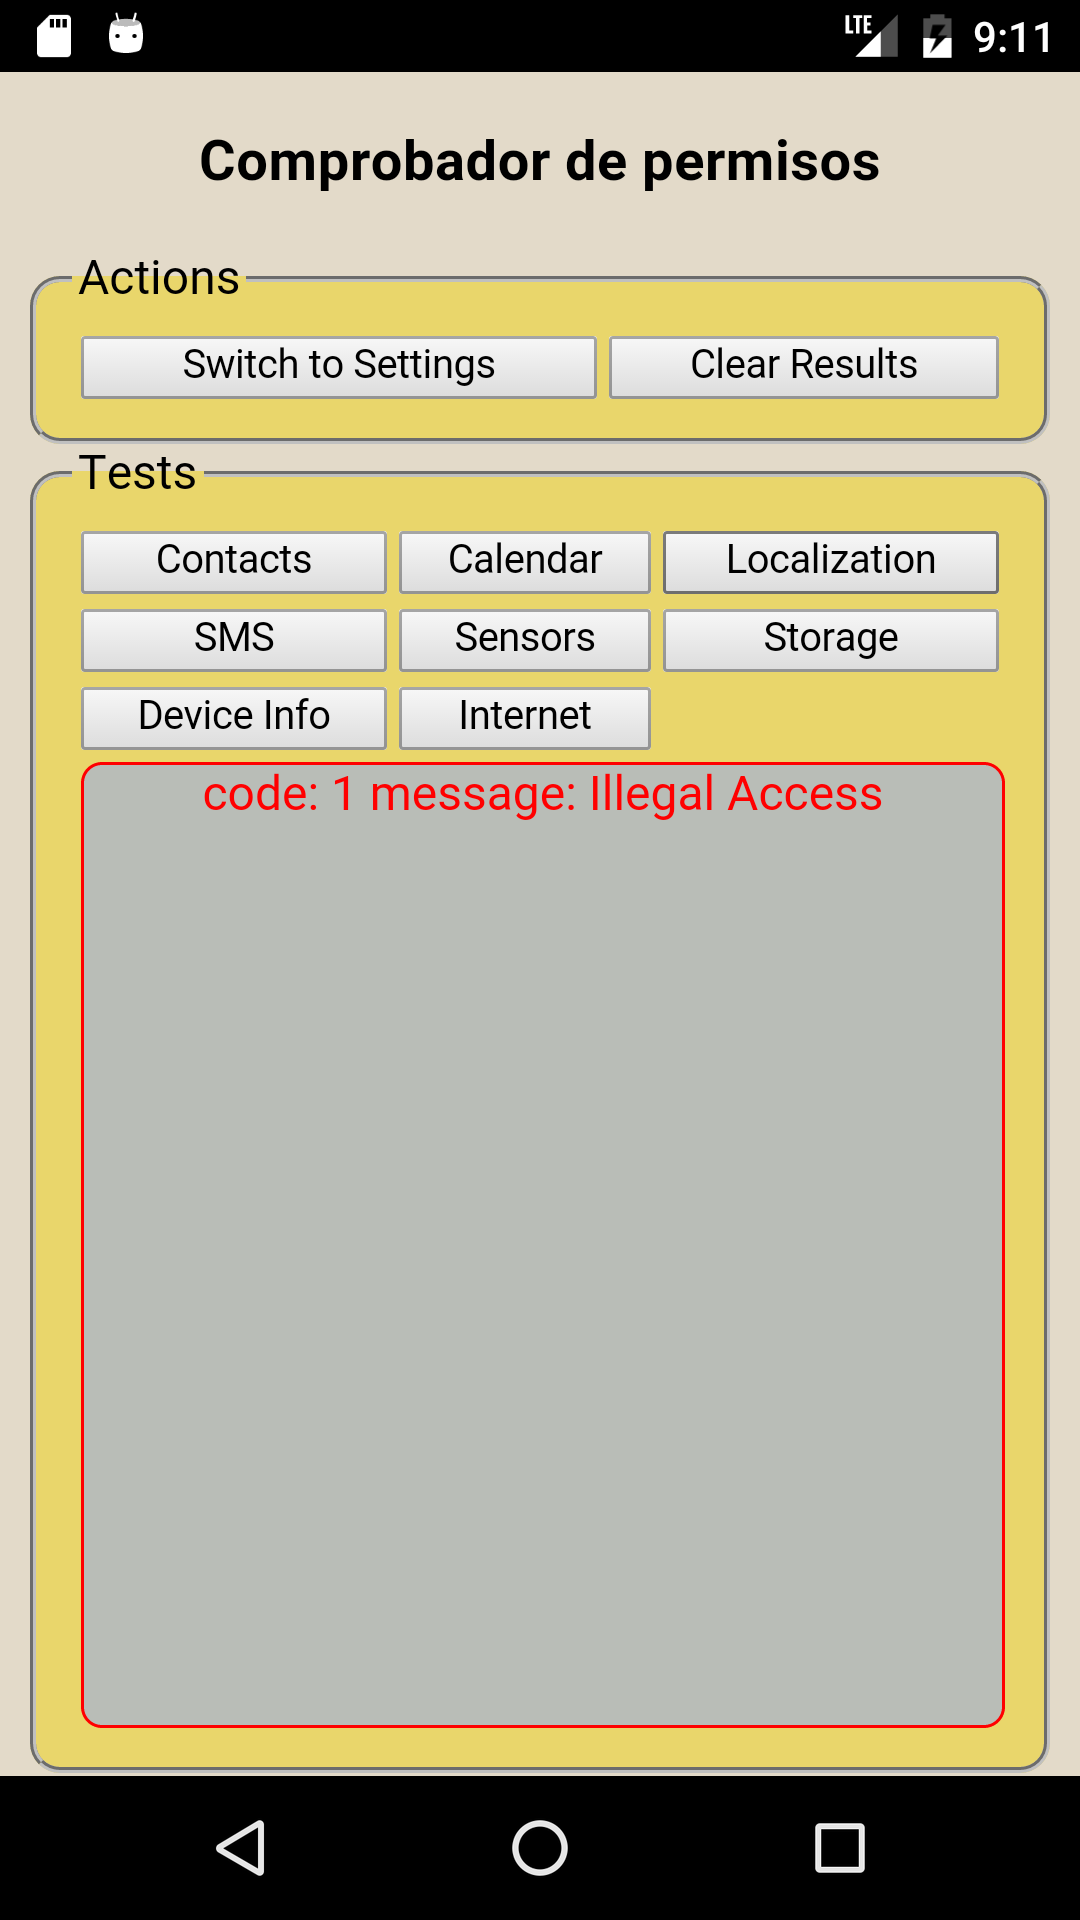
\includegraphics[width=3.75cm]{chapter5/without_location}
		\label{fig:chapter05:without_location}
	\end{subfigure}
	\begin{subfigure}{.24\textwidth}
	    \centering
		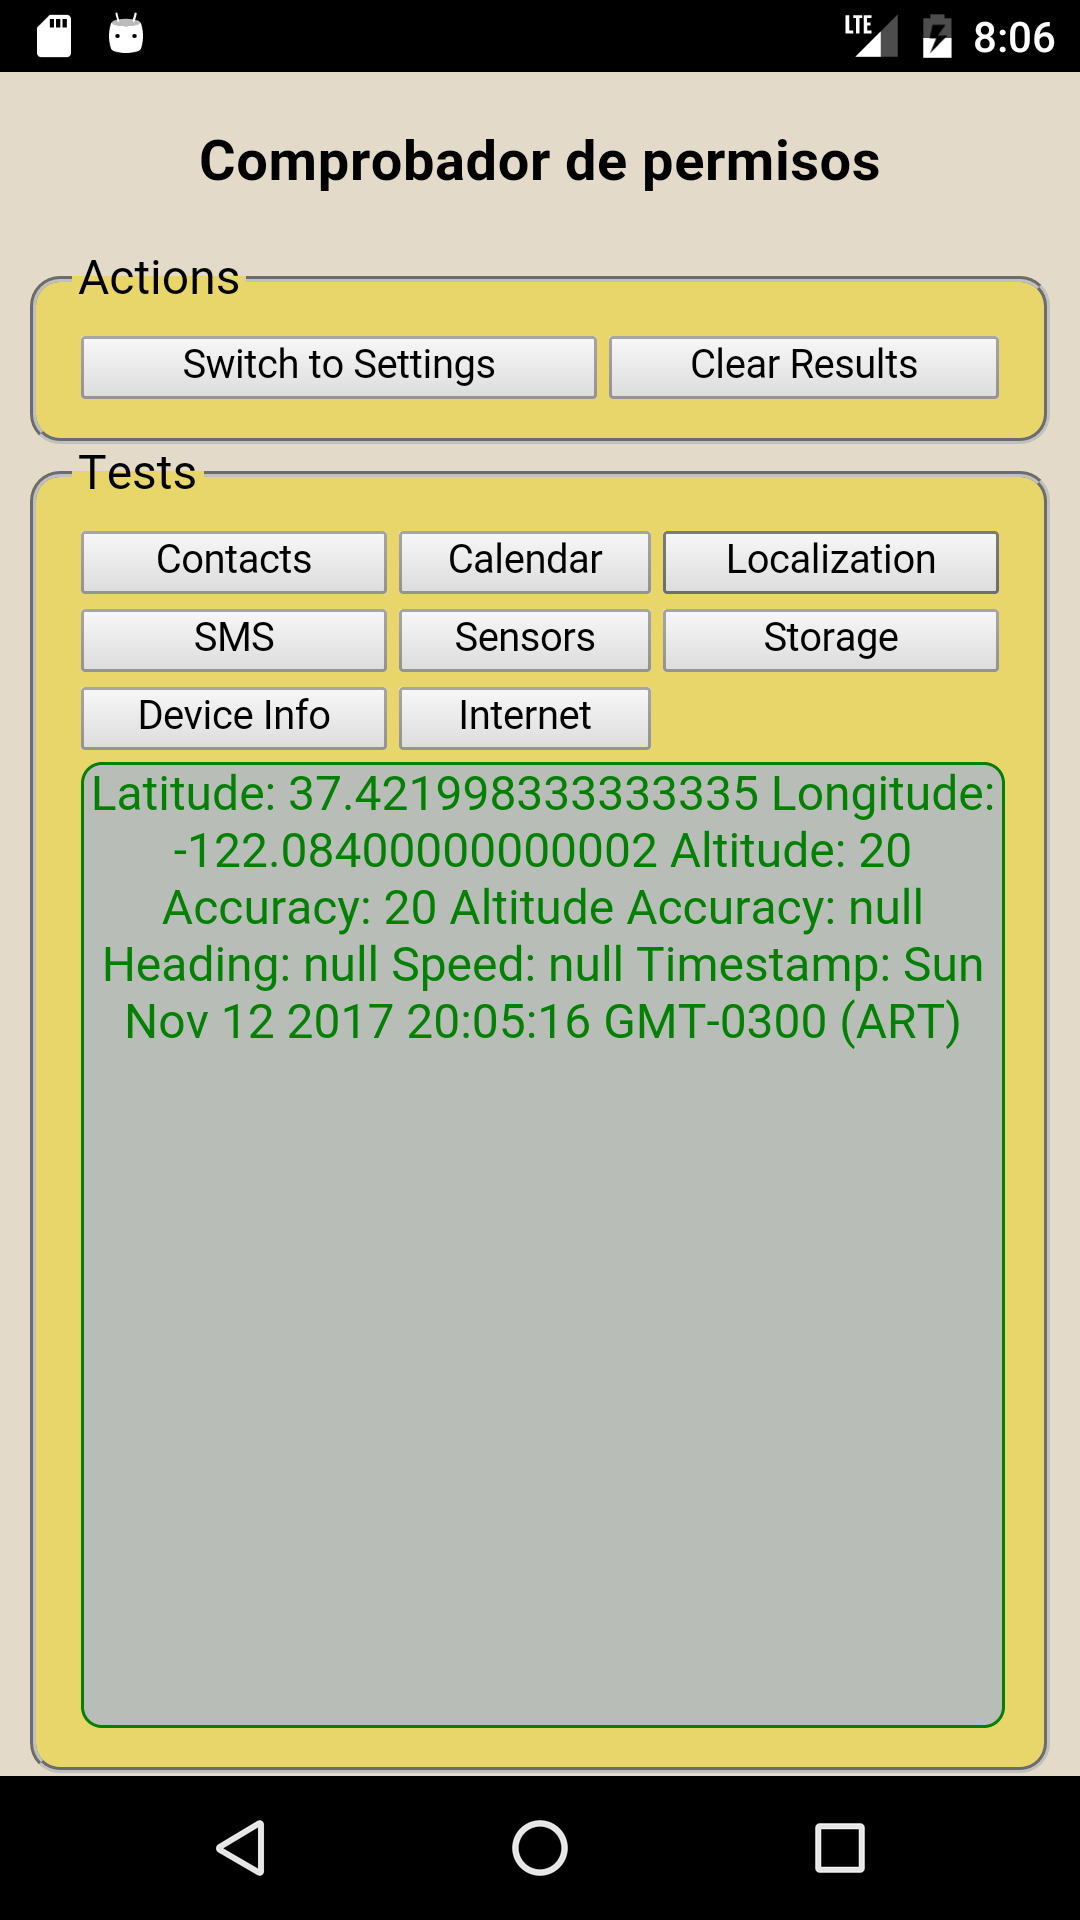
\includegraphics[width=3.75cm]{chapter5/location_success}
		\label{fig:chapter05:location_success}
	\end{subfigure}
	\caption{Testeando la geolocalizaci\'on}
	\label{fig:chapter05:geolocation_test}
\end{figure}\\
\newpage
\subsection*{Almacenamiento}
En iOS no fueron necesarios permisos para poder correr el test.
\textbf{\emph{Plugin:}} \href{https://github.com/gitawego/cordova-screenshot}{cordova-screenshot}\\
\begin{algorithm}
	\begin{algorithmic}[1]
		\STATE Se intenta capturar la pantalla y guardarla en el dispositivo.
	\end{algorithmic}
	\caption{Test de los sensores}\label{alg:chap5_test_storage}
\end{algorithm}
\begin{figure}[!ht]
	\begin{subfigure}{.32\textwidth}
	    \centering
		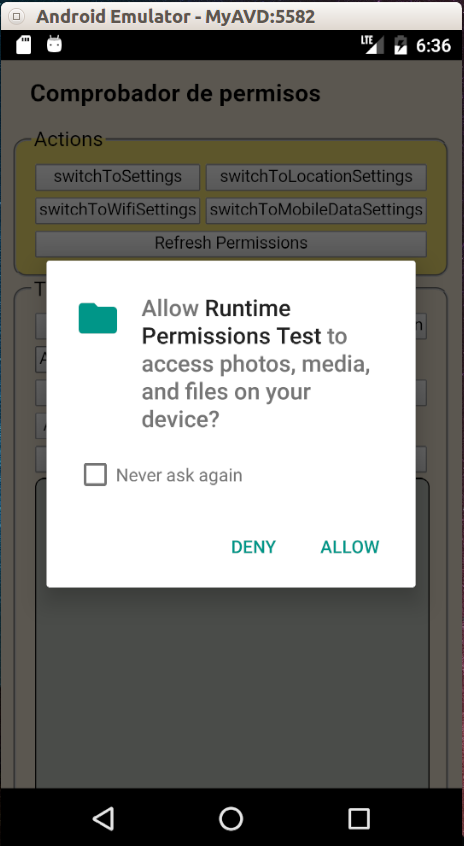
\includegraphics[width=3.75cm]{chapter5/allow_storage}
		\label{fig:chapter05:storage_allow}
	\end{subfigure}
	\begin{subfigure}{.32\textwidth}
	    \centering
		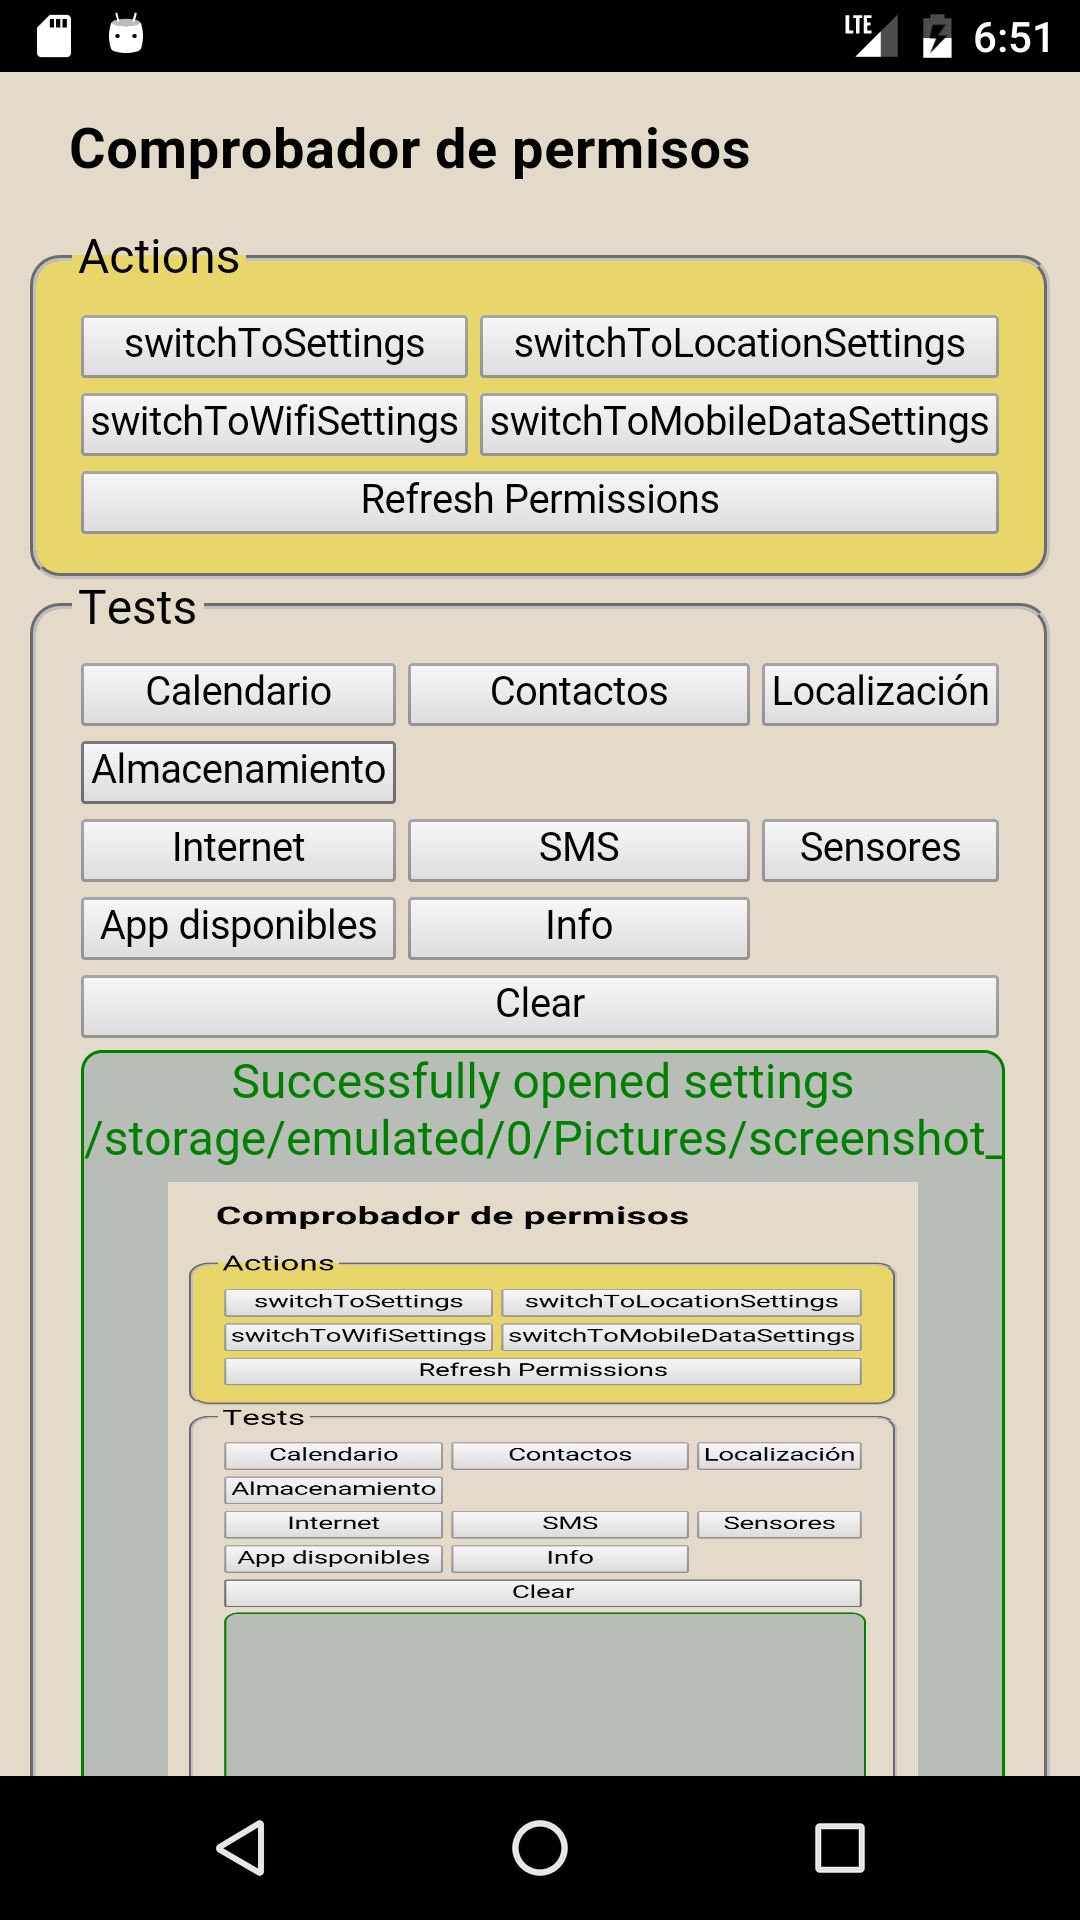
\includegraphics[width=3.75cm]{chapter5/storage_success}
		\label{fig:chapter05:storage_success}
	\end{subfigure}
	\begin{subfigure}{.32\textwidth}
	    \centering
		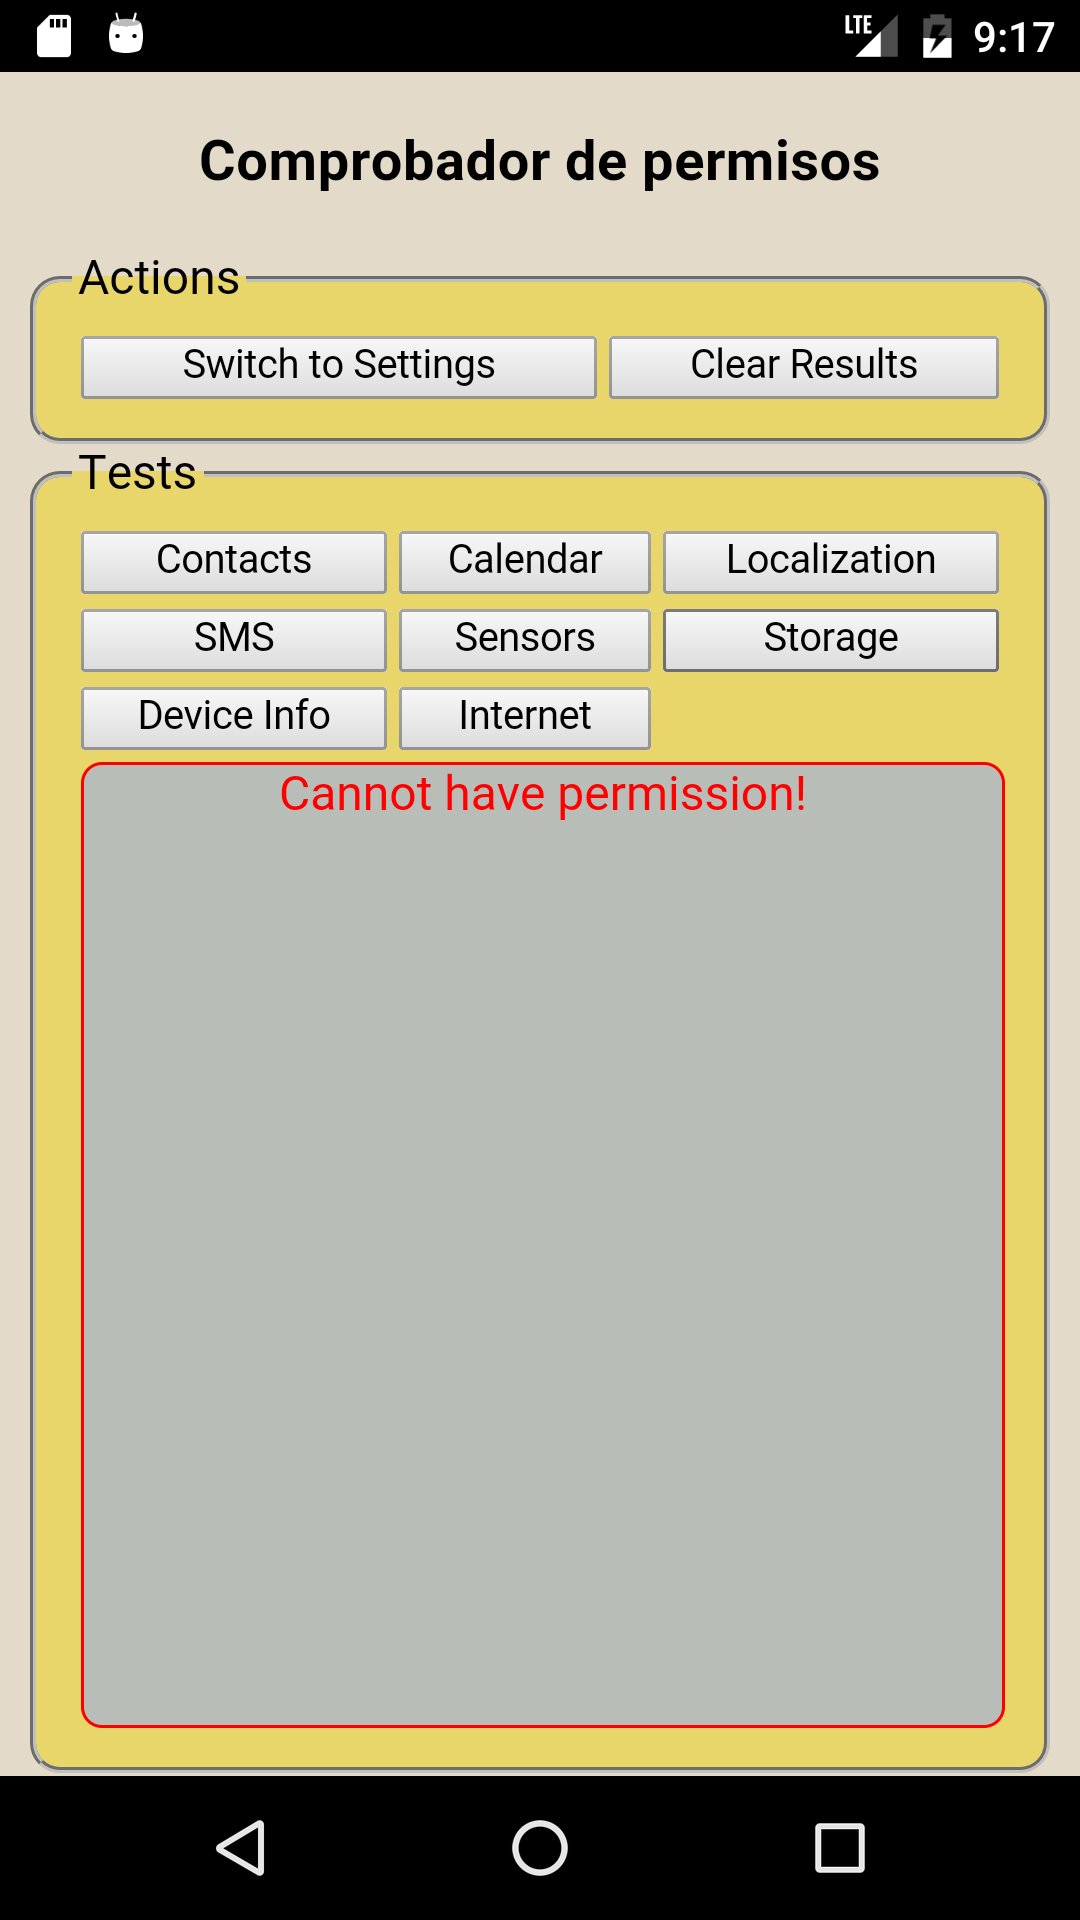
\includegraphics[width=3.75cm]{chapter5/storage_fail}
		\label{fig:chapter05:storage_fail}
	\end{subfigure}
	\caption{Testeando el almacenamiento.}
	\label{fig:chapter05:storage_test}
\end{figure}
\subsection*{SMS}
\textbf{\emph{Plugin:}} \href{https://github.com/floatinghotpot/cordova-plugin-sms}{cordova-plugin-sms v.1}\\
\begin{algorithm}
	\begin{algorithmic}[1]
		\STATE Se inicializan los eventos para recibir SMS. 
		\STATE Se envia un SMS de prueba.
	\end{algorithmic}
	\caption{Test de los permisos de los mensajes SMS}\label{alg:chap5_test_sms}
\end{algorithm}
\begin{figure}[!ht]
	\begin{subfigure}{.32\textwidth}
	    \centering
		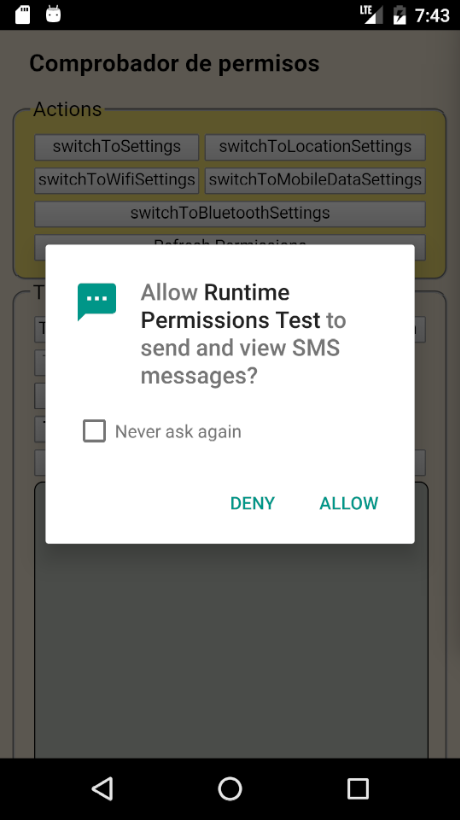
\includegraphics[width=3.75cm]{chapter5/allow_sms_ios}
		\caption{$1^{era}$ vez pregunta si puede acceder a un permiso $peligroso$}
		\label{fig:chapter05:allow_sms_ios}
	\end{subfigure}
	\begin{subfigure}{.32\textwidth}
	    \centering
		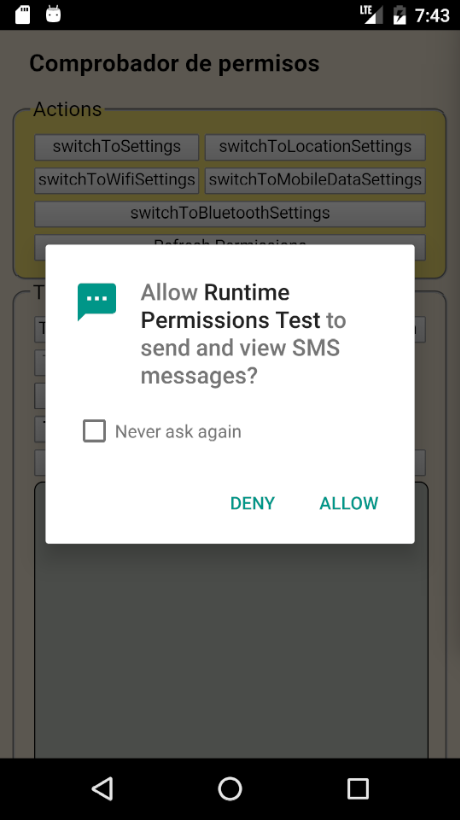
\includegraphics[width=3.75cm]{chapter5/allow_sms}
		\caption{$1^{era}$ vez pregunta si puede acceder a un permiso $peligroso$}
		\label{fig:chapter05:allow_sms}
	\end{subfigure}		
	\begin{subfigure}{.32\textwidth}
	    \centering
		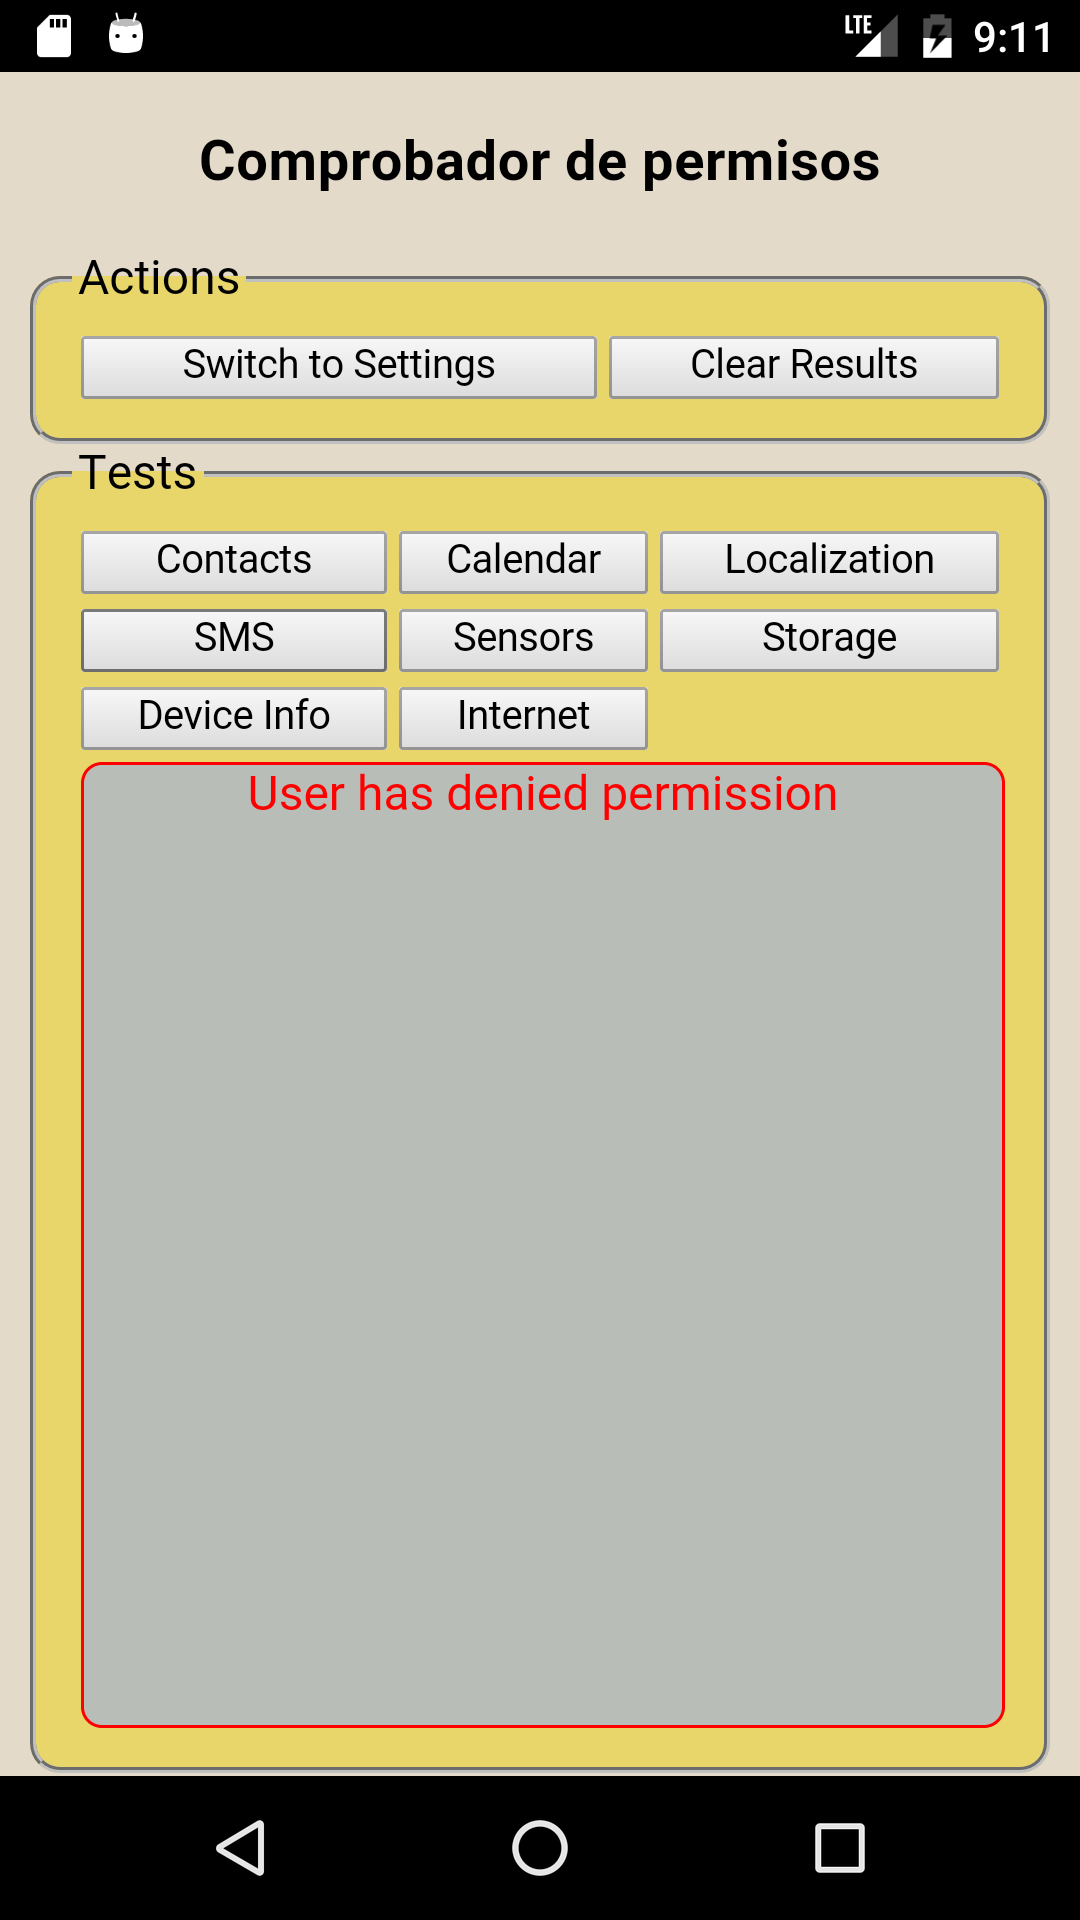
\includegraphics[width=3.75cm]{chapter5/without_sms}
		\caption{Mensaje cuando no se tiene el permiso correspondiente.}
		\label{fig:chapter05:without_sms}
	\end{subfigure}
	\begin{subfigure}{.32\textwidth}
	    \centering
		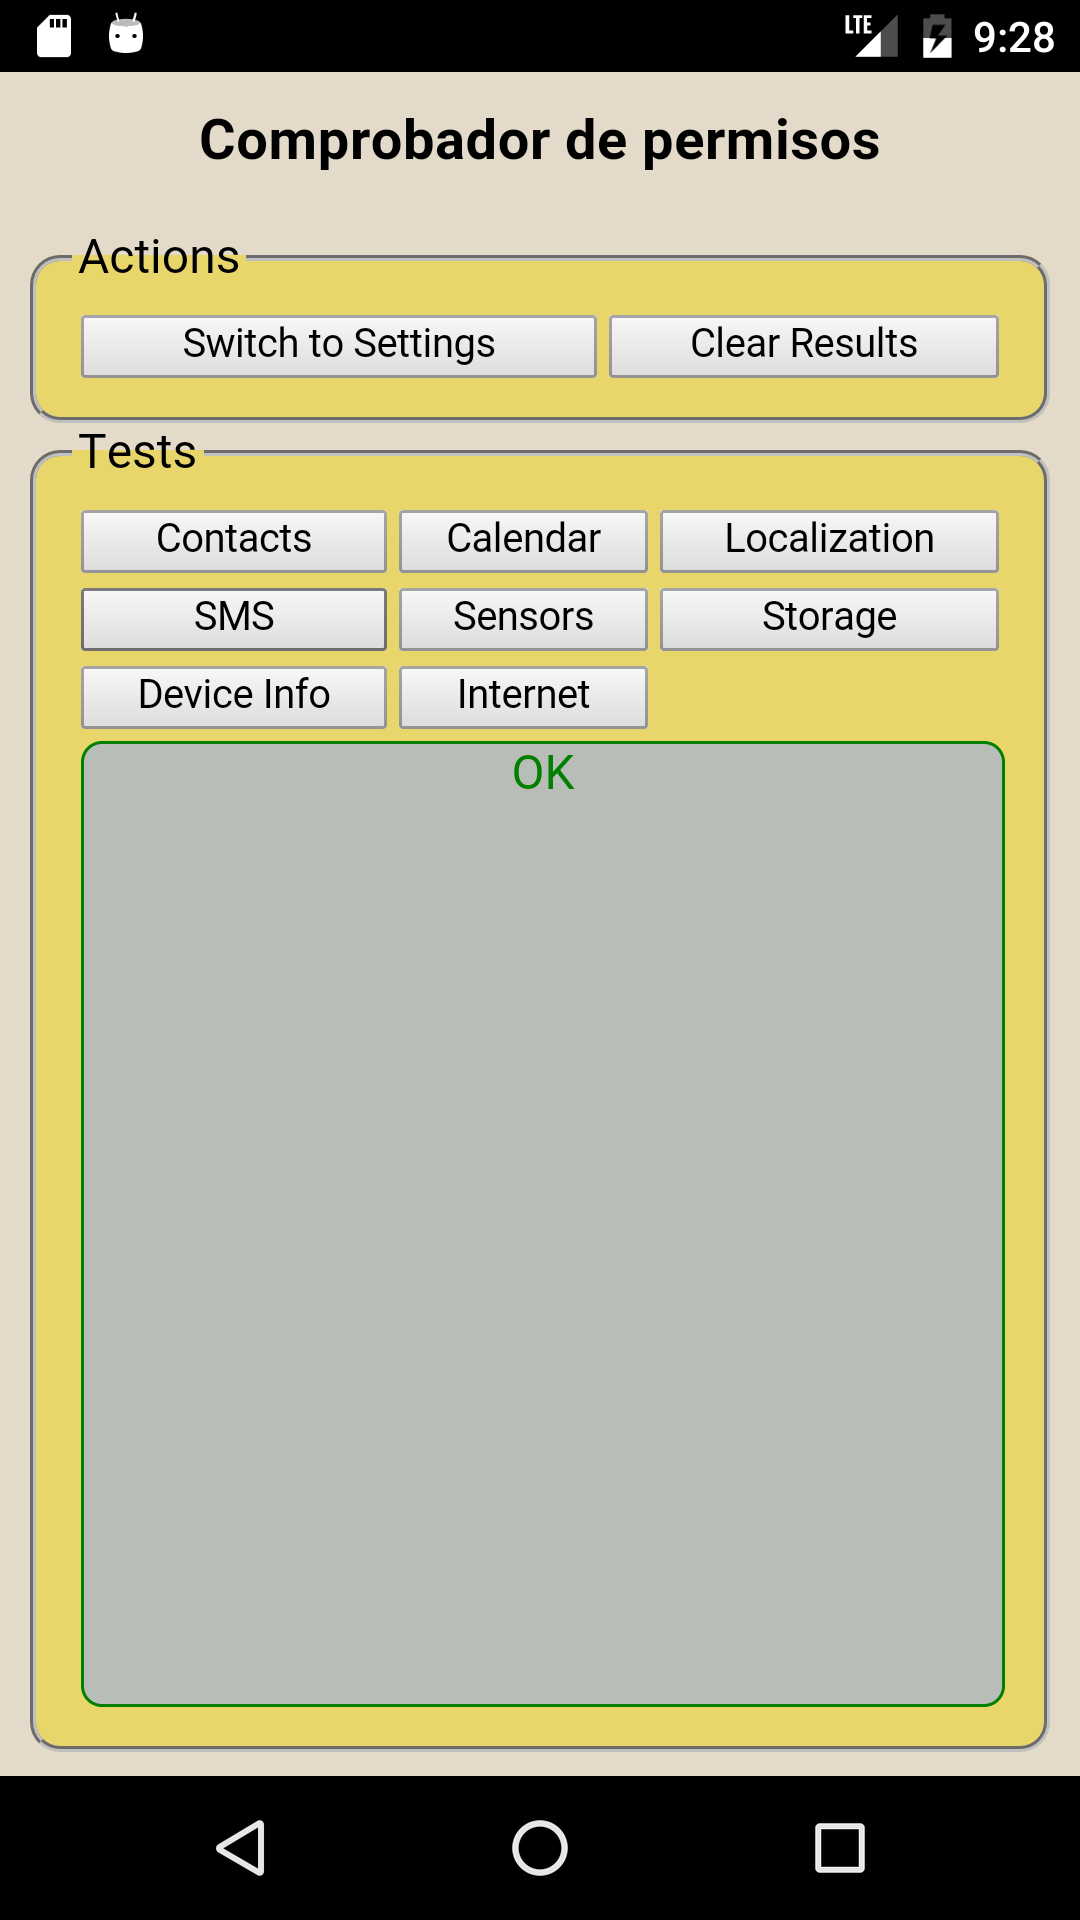
\includegraphics[width=3.75cm]{chapter5/success_sms}
		\caption{Mensaje luego de enviar un sms.}
		\label{fig:chapter05:success_sms}
	\end{subfigure}
	\caption{Testeando los mensajes SMS.}
	\label{fig:chapter05:sms_test}
\end{figure}
En un principio, se quer\'ia agregar al test la funcionalidad de leer los mensajes. Se decidi\'o quitarla ya que a partir de iOS 8 no se pueden acceder a dichos mensajes desde una app instalada por el usuario \cite{foda}. En cambio, en Android si se pueden acceder, siempre que se tengan los permisos correspondientes.
\subsection*{Internet}
\begin{algorithm}
	\begin{algorithmic}[1]
		\STATE se realiza una consulta GET HTTP hacia \href{https://dcc.fceia.unr.edu.ar/sites/all/themes/birthofcool/images/logo-lcc.png}{logo del DCC}
		\STATE se decodifica la imagen (viene codificada en Base64).
		\RETURN un tag \textless IMG\textgreater cuyo \textit{source} es el dato decodificado.
	\end{algorithmic}
	\caption{Test de conexión a internet}\label{alg:chap5_test_internet}
\end{algorithm}
\begin{figure}[!ht]
	\begin{subfigure}{.45\textwidth}
	    \centering
		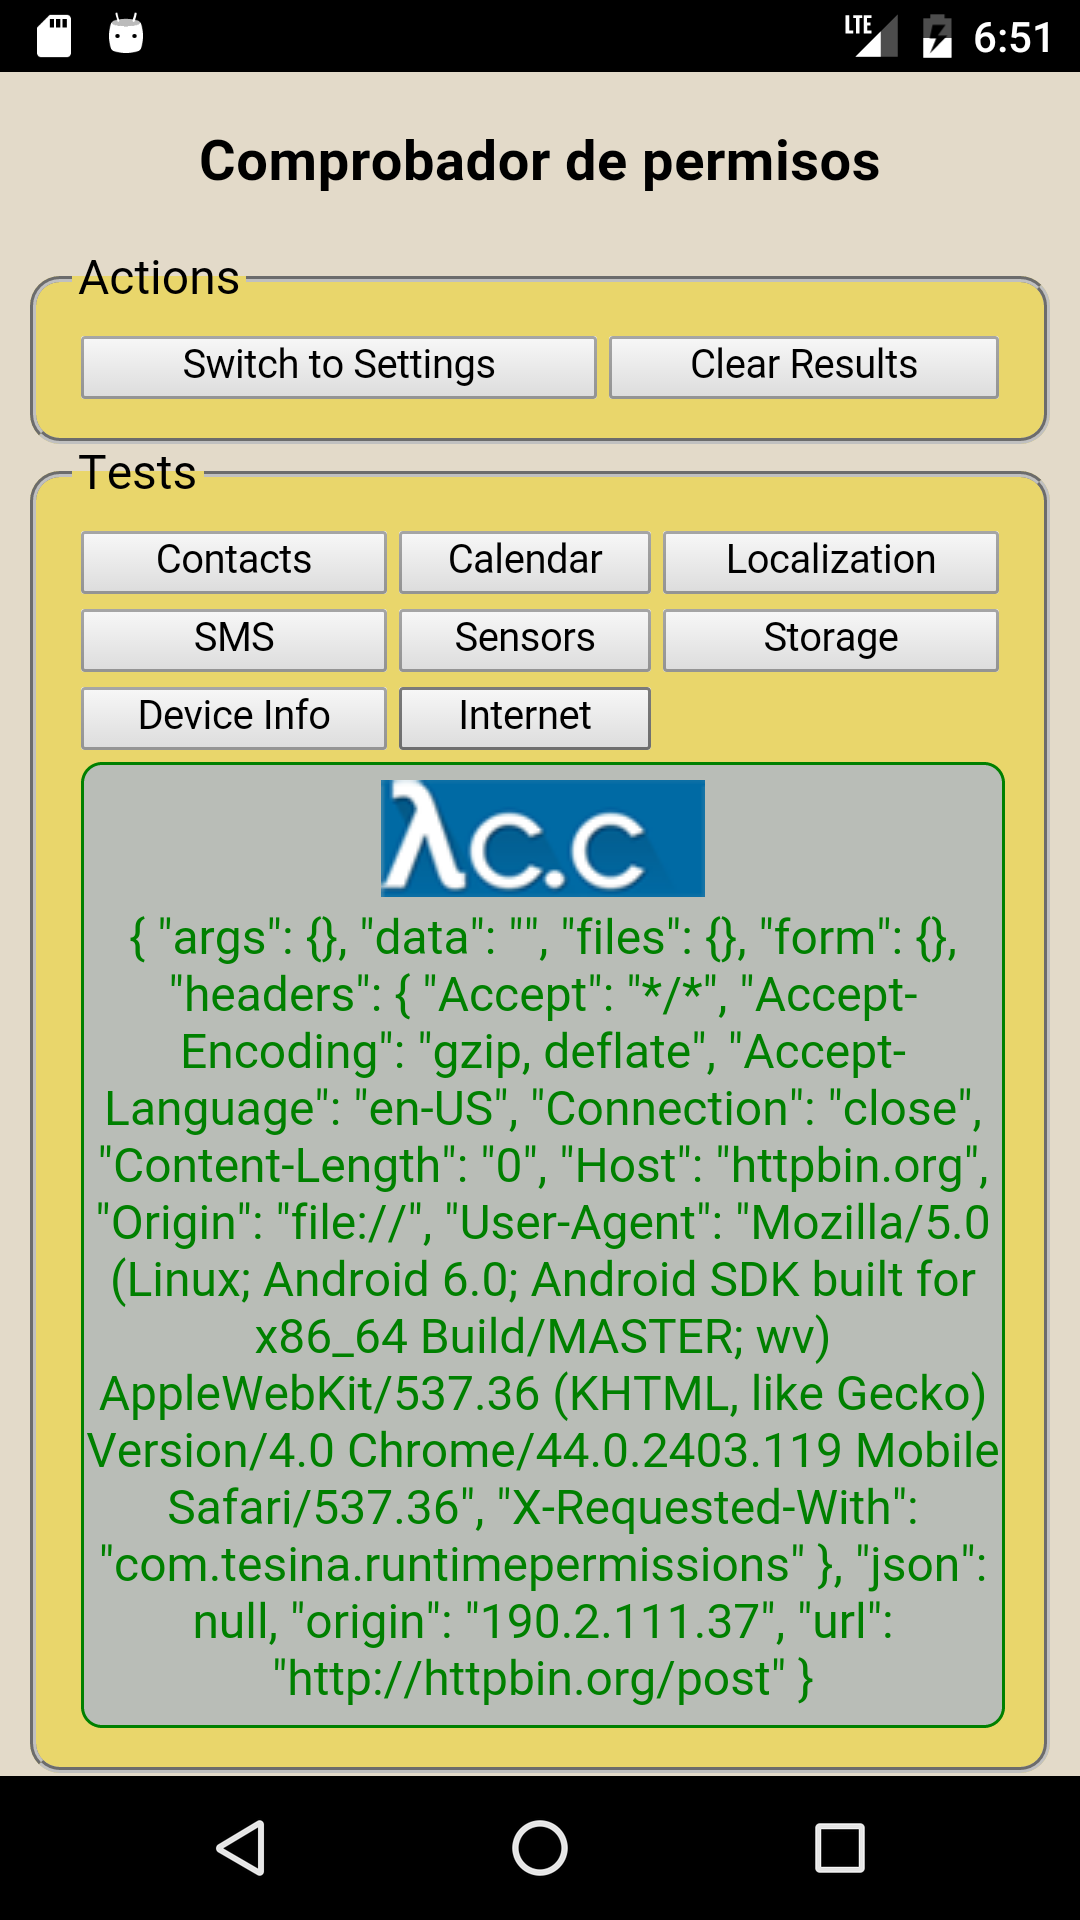
\includegraphics[width=5cm]{chapter5/success_request}
		\caption{Respuesta satisfactoria a la consulta.}
		\label{fig:chapter05:success_request}
	\end{subfigure}
	\begin{subfigure}{.45\textwidth}
	    \centering
		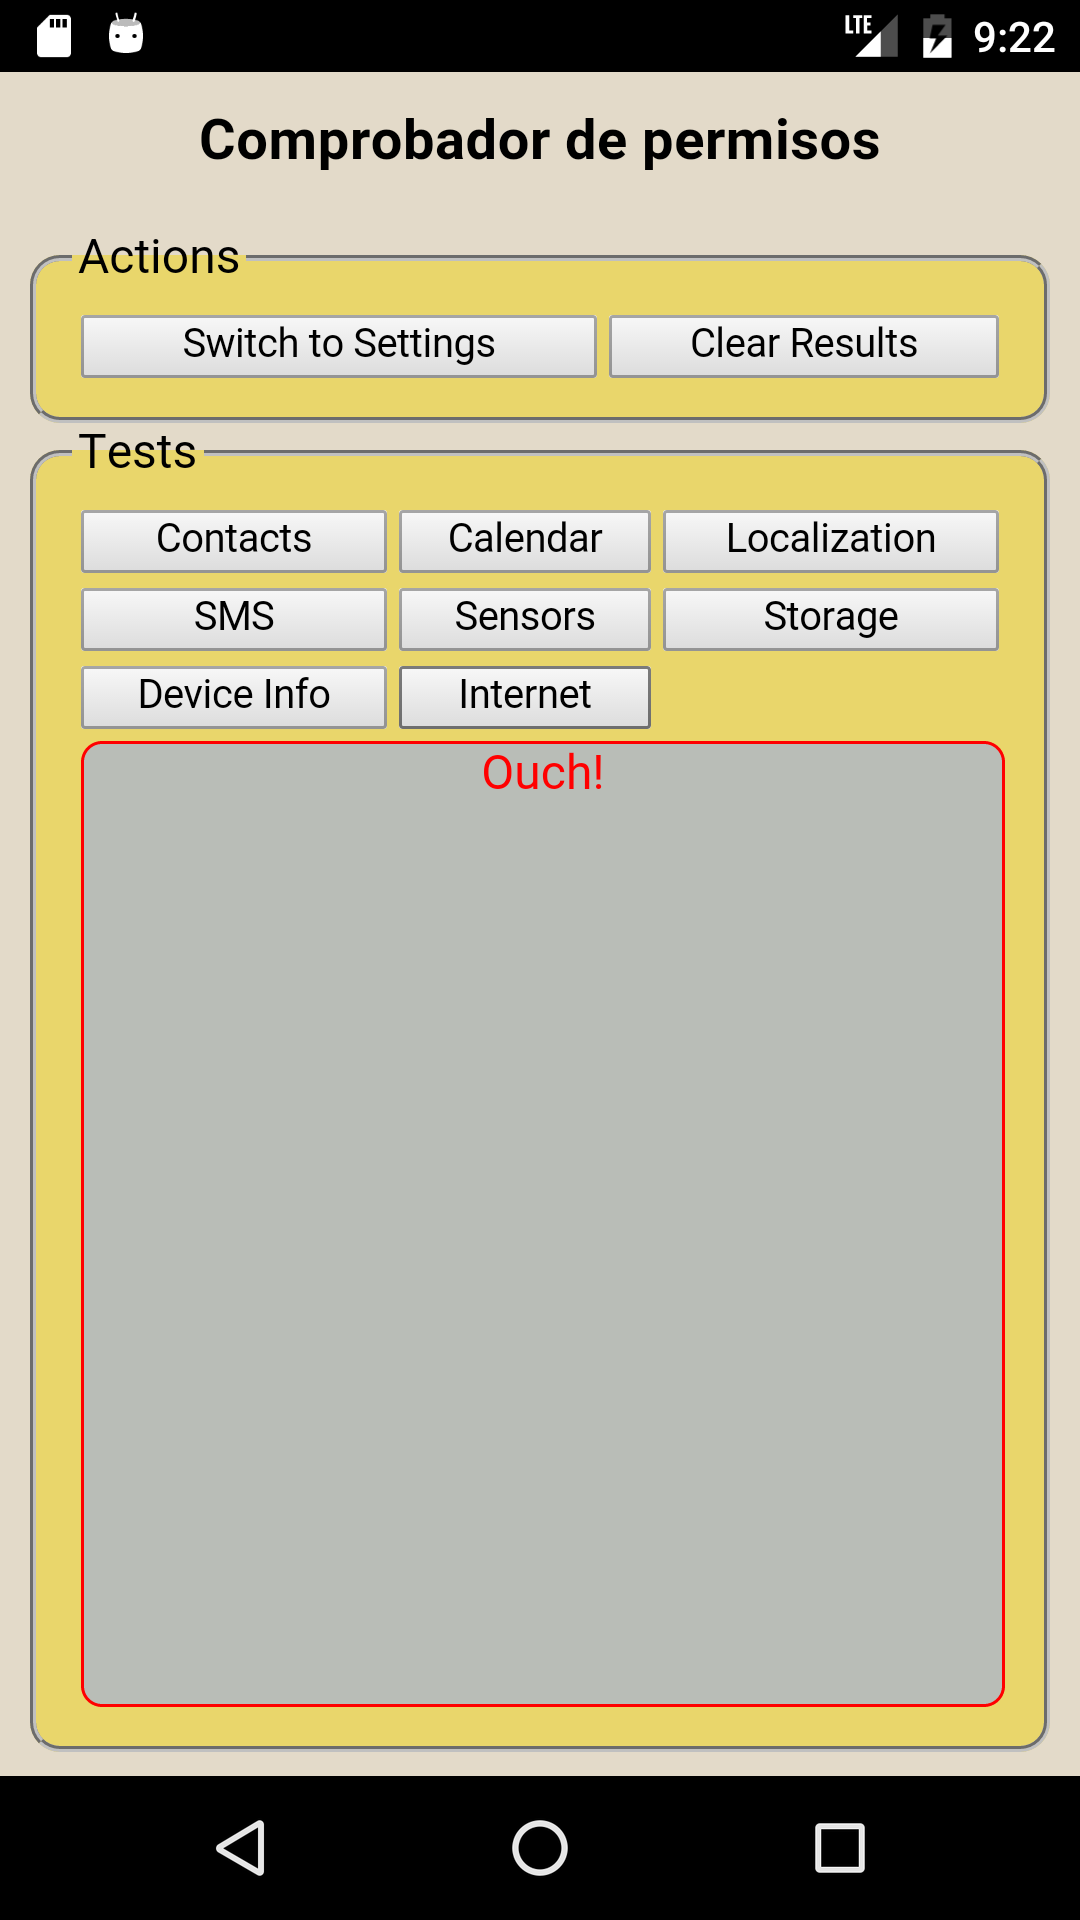
\includegraphics[width=5cm]{chapter5/fail_request}
		\caption{Respuesta erronea a la consulta HTTP.}
		\label{fig:chapter05:fail_request}
	\end{subfigure}
	\caption{Testeando el acceso a internet}
	\label{fig:chapter05:internet_test}
\end{figure}
La decodificacion de la imagen se obtuvo de \href{https://stackoverflow.com/questions/19124701/get-image-using-jquery-ajax-and-decode-it-to-base64/25371174#25371174}{StackOverflow}. Al estar en un emulador, para probar el acceso a internet, se habilitó/deshabilitó la Red Inalámbrica.\\
\newpage
\subsection*{Sensors}
\textbf{\emph{Plugin:}} \href{https://www.npmjs.com/package/cordova-plugin-device-motion}{cordova-plugin-device-motion}\\
\textbf{\emph{Plugin:}} \href{https://www.npmjs.com/package/cordova-plugin-gyroscope}{cordova-plugin-gyroscope}\\
\begin{algorithm}
	\begin{algorithmic}[1]
		\STATE Se inicializa un TIMER con \texttt{5 seg} para detener las mediciones.
		\STATE Se inicia la medici\'on del aceler\'ometro.
		\STATE Se inicia la medici\'on del girosc\'opio.
	\end{algorithmic}
	\caption{Test de los sensores}\label{alg:chap5_test_sensors}
\end{algorithm}
\begin{figure}[!ht]
	\begin{subfigure}{.32\textwidth}
	    \centering
		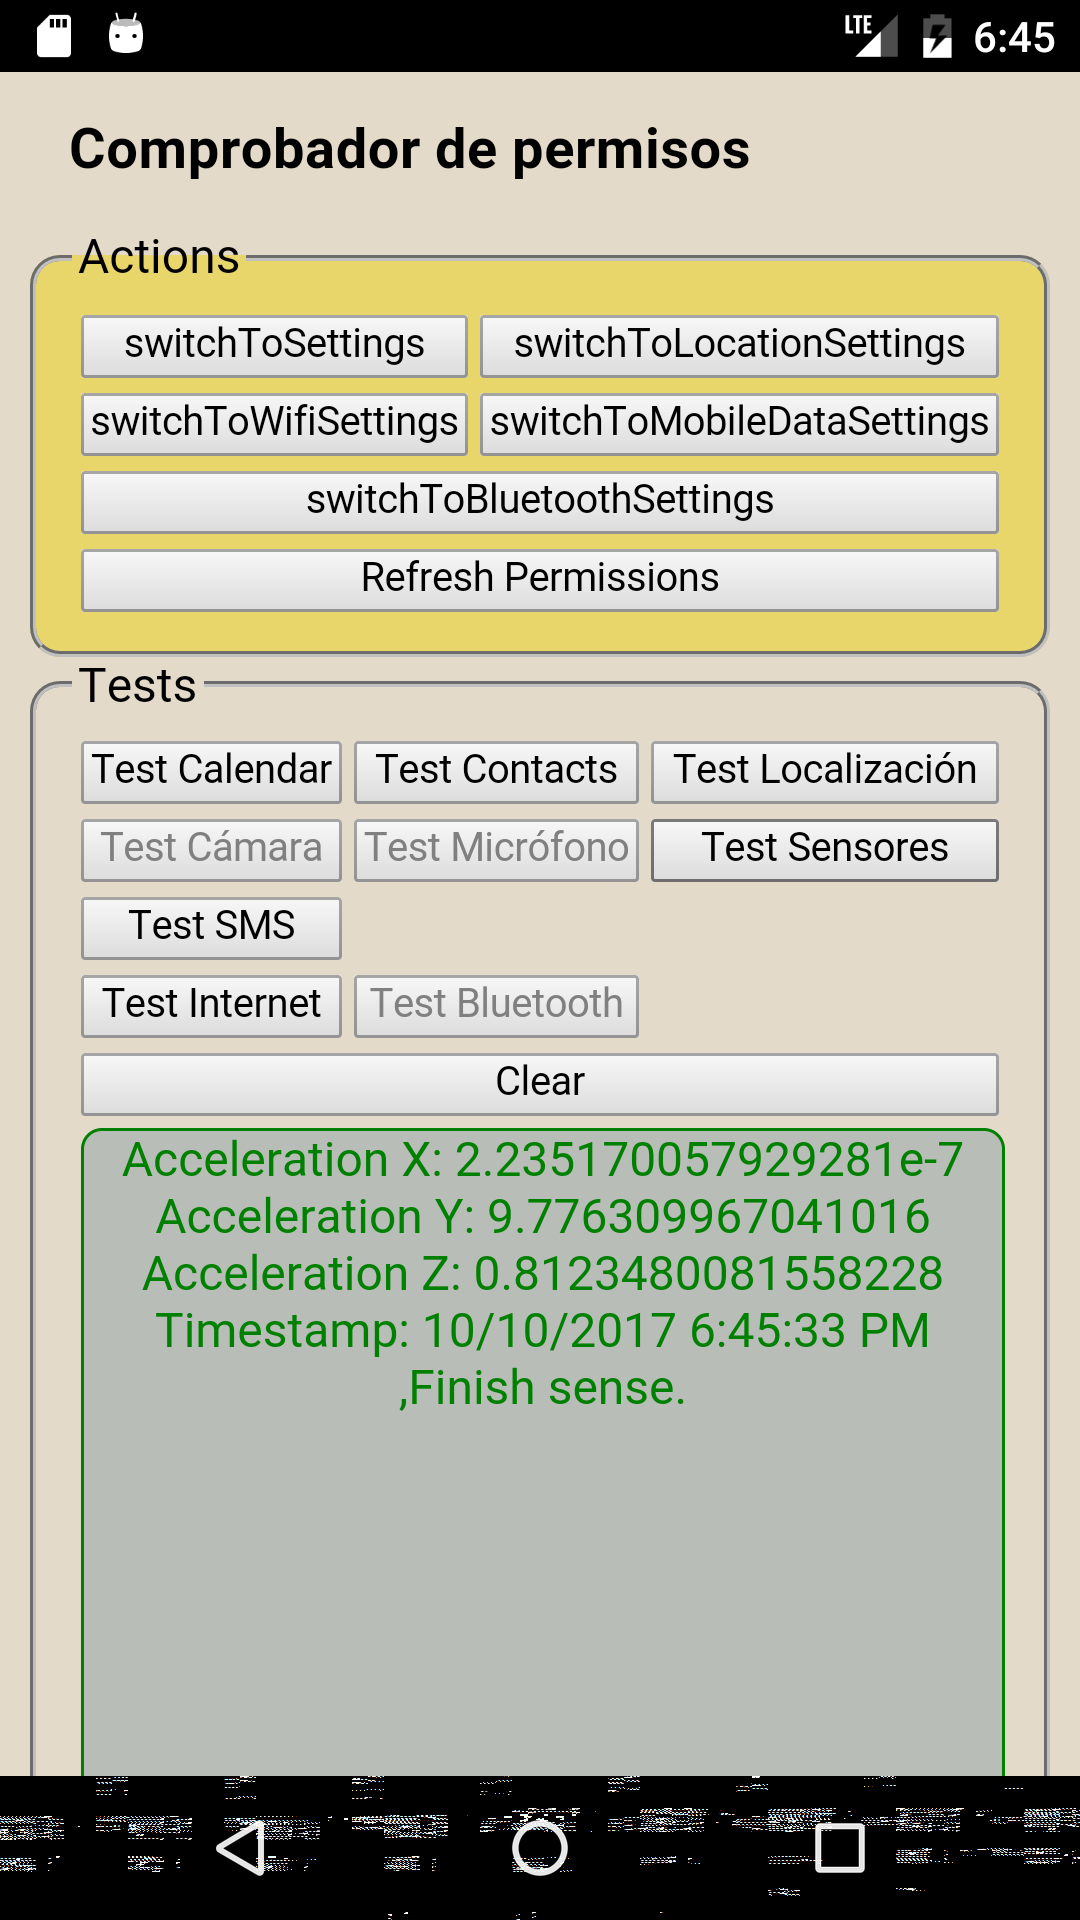
\includegraphics[width=3.75cm]{chapter5/accelerometer_success}
		\caption{Datos medidos}
		\label{fig:chapter05:accelerometer_success}
	\end{subfigure}
	\caption{Testeando los sensores.}
	\label{fig:chapter05:sensors_test}
\end{figure}
En iOS no fueron necesarios permisos para poder correr el test.

\subsection*{AppAvailable}
\textbf{\emph{Plugin:}} \href{https://www.npmjs.com/package/cordova-plugin-appavailability}{cordova-plugin-appavailability}\\
TODO las capturas estan hechas pero no hay nada escrito
No fueron necesarios permisos para poder correr el test.
\subsection*{DeviceInfo}
\textbf{\emph{Plugin:}} \href{https://www.npmjs.com/package/cordova-plugin-device}{cordova-plugin-device}\\
TODO las capturas estan hechas pero no hay nada escrito
No fueron necesarios permisos para poder correr el test.
\subsection*{Batery}
\textbf{\emph{Plugin:}} \href{https://github.com/apache/cordova-plugin-battery-status}{cordova-plugin-battery-status}\\
TODO las capturas estan hechas pero no hay nada escrito
No fueron necesarios permisos para poder correr el test.
\subsection*{Health}
\textbf{\emph{Plugin:}} \href{https://github.com/Telerik-Verified-Plugins/HealthKit}{com.telerik.plugins.healthki}\\
TODO las capturas estan hechas pero no hay nada escrito
No fueron necesarios permisos para poder correr el test.